% 修論の場合は次の行を \documentclass[master]{nagasaki} とすること
\documentclass[master]{nagasaki}
\setcounter{secnumdepth}{4}
\setcounter{tocdepth}{4}
\usepackage{bm}
\usepackage[dvips]{graphicx}
\usepackage{subfigure}
\usepackage{tabularx}
\usepackage{multirow}
\usepackage{amssymb}
\usepackage{array}
\usepackage{amsfonts}
\usepackage{latexsym}
\usepackage{amsmath}
%%%%%%%%%%%%%%%%%%%%%%%%%%%
\title{ニュース音声におけるインデクシングのためのアンカーの発話区間検出と音声認識精度の向上}         % 論文題目
\author{野崎 大智}            % 著者
\teacher{松永 昭一 教授} % 指導教官名
\id{52117321}            % 学籍番号
\date{\today}
\date{平成30年度}        % 年度
%%%%%%%%%%%%%%%%%%%%%%%%%%%%%
\begin{document}
\maketitle
\clearpage
\pagestyle{headnombre}
\pagenumbering{roman}
\tableofcontents
\listoffigures
\listoftables
\clearpage
\pagestyle{headings}
\pagenumbering{arabic}
%%%%%%%%%%%%%%%%%%%%%%%%%%%%%
% 以下本文
\chapter{研究背景}

\section{研究背景}
近年、通信・放送業界では地上デジタル放送の開始や、新たな高速通信規格の誕生など、通信ネットワークの急速な発達が見られる。それに伴い、誰もがテレビやパソコンだけでなくスマートフォン・タブレットなど様々なデバイスを通して手軽に膨大な量の音声・映像データを入手し、好きな時に好きな場所で視聴することが容易な時代となった。そこで、映像・音声データに話者や内容のインデックスの情報が付与されていれば、必要な部分のみを容易に検索、視聴ができる。しかし、世の中には膨大な量の映像・音声データが存在するため、それら全てに人手でインデクスを付与することは事実上不可能である。そこで、自動的にインデクシングすることが望まれる。\par
自動でインデクシングを行うためには、映像・音声データ内の発話区間、発話者、発話内容の特定が必要である。これらを推定する技術のことをダイアライゼーションと呼び、本稿はこの技術の実現を目指す。\par
本稿では世の中に存在する映像・音声データの中で、ある特定の人物に情報が集中する形式で行われるニュース番組に着目した。

\vspace{0.2in}\noindent{\textbf{\underline{ニュース番組の特徴}}}
\begin{itemize}
\item 30分程度のニュース番組の中で複数の多様な話題がある
\item 1人または複数のアンカーおよび天気予報士など複数の話者が存在する
\item 話者情報(話者数、性別、話者の声質など)および発話区間が未知である
\item 対話が少ない
\item アンカーは連続で発話することが多い
\end{itemize}

\noindent このようなニュース番組において、ニュースの話題にインデクシングが行われていることは必要な話題の検索に重要である。ここで、アンカーとは司会役のアナウンサーのことであり、ニュース番組は主にアンカーを中心として進行する。アンカーの特徴は以下の通りである。

\vspace{0.2in}\noindent{\textbf{\underline{アンカーの特徴}}}
\begin{itemize}
\item 発話数が多い
\item ニュース番組の司会および話題の切り替えを行う
\item ニュース番組の全体にわたって発話している
\end{itemize}

\noindent このため、ニュース番組ではアンカーの発話に情報が集中しており、インデクシングに重要な情報を持つ。つまり、アンカーの発話区間を検出、音声認識はニュース番組のダイアライゼーションの実現に有効であると考えられる。

\section{研究目的}
特定話者の発話検出には話者特徴量(i-vector)が一般的に用いられている。また、音声認識においても認識対象の話者ごとに音声認識システムを適応させることで音声認識精度の向上が確認されている。しかし、短い発話からは話者の識別に必要なi-vectorを抽出できないことが確認されており\cite{panaiv}、アンカーの発話の誤検出、音声認識精度の低下につながる可能性がある。そこで、短い発話のi-vectorの抽出精度を向上することによって、アンカーの発話区間検出精度、音声認識精度の向上が見込めると考えた。\par
本稿では、前後の発話区間が同一話者の発話である可能性が高いとき発話区間を結合し、長い発話を擬似的に作成した。これによって短い発話のi-vectorの抽出精度向上を目指し、アンカーの発話区間検出と音声認識への有意性を検証した。検証を行なった結果、従来と比較してアンカーの発話区間検出精度が9\%、音声認識精度がhogehoge\%の向上を実現した。これにより、i-vectorの抽出において発話区間を結合し擬似的に長い発話を作成することにより、アンカーの発話区間検出、音声認識への有意性を示した。

\section{論文構成}
次章以降における本論文の構成は、まず2章で本実験で用いるシステム、アルゴリズムの概要について説明を行う。次に3章では、i-vectorの性質と評価対象であるニュース番組音声の調査を行う。4章ではi-vectorを用いたアンカーの発話検出手法と音声認識の先行研究について述べ、問題提起を行う。5章では本研究で提案するアルゴリズムの説明を行う。6章では提案手法を用いた発話区間の結合、i-vectorを再抽出を行い、アンカーの発話区間検出精度、音声認識精度への効果を検証する。7章では本研究において検証された実験の結果を元に結論を述べる。

  % 研究背景
\chapter{理論的背景}

\section{音源識別}
\section{音源分離システムの概要}
\renewcommand{\labelenumi}{(\arabic{enumi})}
音響データの中にはさまざまな音源種別(声、音楽、雑音等)の音が混在している。音源識別とは、音響データ中に含まれる音源種別を自動的に識別することである。ここでの処理は、音響データのスペクトル解析を行い、音響特徴パラメータを求め、あらかじめ用意した各音源種別の音響特徴パラメータの分布と比較することで音源種別を識別する。\par
本システムでは、ニュース番組の音声データに音響特徴パラメータを用いた音源識別\cite{shimae_9} を用い、音声データ中の音源種別を以下の4つに分類した。

\begin{enumerate}
\item 音声区間: アナウンサーやインタビューの声
\item 音楽区間: オープニングやエンディングなどの音楽、BGM
\item 背景雑音区間: 自動車走行音や鳥の泣き声、喧騒
\item 無音区間: 音量が極めて小さい区間
\end{enumerate}

また、音源識別システムは音響データを各種別へ識別するための音響特徴パラメータの分布に8混合のガウス分布を用いている。本研究の音響特徴パラメータを表\ref{table:feature_devide_audio}に示す。
\begin{table}[H]
  \begin{center}
    \caption{音源識別のための音響特徴パラメータ}
    \label{table:feature_devide_audio}
    \begin{tabular}{|c|c|} \hline
      スペクトルの変化 & スペクトルの傾き\\ \hline
      白色雑音との近さ & ピッチ  \\ \hline
      パワー & 中心周波数 \\  \hline
      中心周波数のバンド幅 &   \\ \hline
    \end{tabular}
  \end{center}
\end{table}

以降、音源識別のためのスペクトル解析と音響特徴パラメータについて説明する。\par


\subsection{スペクトル解析}
音響データのスペクトル解析の手法として最も一般的に利用されている方法は、短時間フーリエスペクトル分析がある。この方法は、音響データから連続する数10ms 程度の時間長の信号区間を切り出し、切り出された信号が定常性(一定周期で繰り返す)と仮定して、スペクトル解析を行う。\par
スペクトル解析の流れは以下の通りである。

\begin{enumerate}
\item フレーム化処理:与えられた信号$s(n)$ に長さ$N$ の窓関数を掛けることで以下のような信号系列$s_\omega(m; l)$を取り出す。
\begin{equation}
S_w(m;l)=\sum_{m=0}^{N-1}\omega(m)s(l+m)\qquad(l=0,T,2T,\cdots), \notag
\end{equation}

ここで、添え字$l$は信号の切り出し位置に対応している。すなわち、$l$を一定間隔$T$で増加させることで定常とみなされる長さ$N$の信号系列$s_\omega(n)\quad (n=0,1,\cdots,N-1)$が間隔$T$で得られる。この処理をフレーム化処理と呼び、$N$をフレーム長、$T$をフレーム間隔と呼ぶ。また、窓関数とは、ある有限区間以外で0となる関数であり、フレーム化されたデータに対して重みをつける関数である。フレーム化処理を行う場合、離散的なデータの繋ぎ目においての信号の急激な変化の影響を和らげるため、原則として窓関数をかけなければならない。代表的なものとして音声信号だけに有効なハニング窓と、音声信号以外にも様々な信号にも有効なハミング窓がある。

\begin{equation}
\label{da1}
ハニング窓:\omega(n)=0.5-0.5\cos(\frac{2\pi n}{N-1}).\qquad(n=0,1,\cdots,N-1) \notag
\end{equation}

\begin{equation}
\label{da2}
ハミング窓:\omega(n)=0.54-0.54\cos(\frac{2\pi n}{N-1}).\qquad(n=0,1,\cdots,N-1) \notag
\end{equation}

\item スペクトル分析(離散時間フーリエ変換、高速フーリエ変換):フレーム化処理によって得られた信号系列の短時間フーリエスペクトルは、離散時間フーリエ変換により以下の式で与えられる。
\begin{equation}
S(n)=\sum s_\omega(n)e^{-j2\pi \frac{nk}{N}}, \qquad (k=0,1,\cdots,N-1) \notag
\end{equation}

離散フーリエ変換(DFT) は、離散的なデータをフーリエ変換する際に、通常のフーリエ変換の無限区間積分を有限の和で書き換えたもので、時間領域、周波数領域ともに離散化されたフーリエ変換のことであり、時間領域の表現を周波数領域における表現に変換する。また、逆に周波数領域の表現を時間領域の表現に変換する、つまり元の音響データに戻す変換を離散フーリエ逆変換(IDFT) と呼び以下の式で与えられる。

\begin{equation}
S(n)=\frac{1}{N}\sum S(k)e^{j2\pi \frac{nk}{N}}. \qquad (k=0,1,\cdots,N-1) \notag
\end{equation}

実際の信号処理過程では、離散的フーリエ変換(DFT) をその高速算法である高速フーリエ変換(FFT) を用いて実行し、当該音声区間のスペクトル表現とすることが一般的である。高速フーリエ変換は式(\ref{da1}),(\ref{da2}) の$N$ が$2^n$ 個であるとき、その処理を高速にできる性質がある。フーリエ変換の式には、

\begin{equation}
S\prime(n)=S(e^{j\frac{2\pi}{n}k})=\sum s_\omega(n)e^{-j2\pi \frac{2\pi}{N}kn}, \qquad (k=0,1,\cdots,N-1) \notag
\end{equation}

なる複素系列$S\prime(k)$が音声スペクトル表現として最も一般的に用いられる。

\item パワースペクトルの算出:音響信号の離散パワースペクトル系列は、離散スペクトル系列から式(\ref{da3}) で表される。

\begin{equation}
\label{da3}
|S^\prime(k)|^2=\frac{1}{N}[\operatorname{Re}\left\{S^\prime(k)\right\}^2+\operatorname{Im}\left\{S^\prime(k)\right\}^2].
\end{equation}

この2乗値のパワースペクトル$|S^\prime(k)|^2$を特徴量として扱っている。音響信号に高速フーリエ変換を施すと、時間表現(縦軸:パワー、横軸:時間) から周波数表現(縦軸:振幅、横軸:周波数)へと変換できる。しかし、実際には縦軸を周波数、横軸を時間としたグラフがよく使用されており、このようなグラフをスペクトログラムという。スペクトログラムは音声を視覚化したものであり、声紋とも呼ばれる。

\end{enumerate}\par

\subsection{音響特徴パラメータ}
本研究で使用する7つの音響特徴パラメータについて述べる\cite{shimae_10}

\begin{enumerate}
\item スペクトルの変化\par
動的特徴量を連続するスペクトルのフレーム間の変化量として取り出す。音響信号のスペクトル分析した連続するフレームにおいて、あるフレームとその一定時間後のフレームとのパワースペクトルの差分によりスペクトルの変化量を得て、そのスペクトルの差分を一定時間足し合わせたものとしている。スペクトルの変化量によって比較する利点は、音声の識別に有利であり音声に比べて背景雑音のほうがスペクトルの変化量が大きく、無音のほうがスペクトルの変化量が小さいということである。

\item スペクトルの傾き\par
あらかじめ人手により作成したラベルにより音響データの各区間を各種別(音声、音楽、背景雑音、無音)に振り分け、それぞれに対してスペクトル分析を行い、パワースペクトルを取り出し、各種別内において集められたパワースペクトルの分布を求めることで各種別において傾き値を得る。この傾き値を基に、与えられた音響ファイルから次々に得るパワースペクトルと各種別の学習データとの特徴パラメータの分布の類似度を比較する。この最小単純形は、パワースペクトルにおける一次回帰直線の傾きを比べることと同じである。傾きによって比較する利点は、有色系の音のほうが白色雑音よりも傾きが大きいので、音声と音楽と無音の識別に有利である。

\item 白色雑音との近さ\par
パワースペクトルより一次回帰直線からスペクトル波形の切片を求めることで入力信号の白色性の度合を計測する。この白色雑音との近さによって比較する利点は、背景雑音のような定常的に混入した雑音は白色性が高いため、これらの識別ができるこということである。

\item ピッチ\par
有声音源の繰り返し周期、いわゆるピッチ(基本周波数)の変化を調べることで、音源の変化を知ることができ、音源の特定のパラメータである。周波数分析によりピッチを求め、学習データと比べることで音源の特定に用いる。

\item パワー\par
時間領域の分析だが、音響信号のような非定常的な信号に対して、変化していく信号の大きさにうまく追随するような比較的短い区間に音響データを区切り、その区間の信号$xl(n)$に対してエネルギー$E(l)$ を定義する\cite{shimae_11}。
\begin{equation}
E(l)=\sum_{n=0}^{N-1}\left\{x_l(n)\right\}^2. \notag
\end{equation}
ここでは、整数$N$ は窓の中に含まれる音響信号の数である。\par
利点としては、測定が簡単であり、音声認識における有色系の音の区間の抽出にもよく用いられることから、有音と無音の区別に有利である。

\item 中心周波数\par
抽出したパワースペクトルにおいて、無音の場合は右下がりに傾斜しているが、有音の場合は傾斜の途中で膨らみまたは突起が発生する。その突起がもっとも大きく発生している周波数帯の中心部分の周波数を中心周波数として定義している。これは有音と無音の識別に効果がある。

\item 中心周波数のバンド幅\par
中心周波数を含む膨らみ、あるいは突起の始まりと終わりによる周波数帯の長さをバンド幅として定義する。音声は一定の周波数を含むことが多いためそのバンド幅はある程度の大きさになることが考えられるが、雑音はあまり多くの周波数を含まないものから白色性が高く幅広い周波数を含むものまで様々であり、その違いから音声と雑音の特定に有効である。
\end{enumerate}\par


\section{i-vectorの概要}
近年の話者認識システムの多くは i-vector\cite{iv}に基づいて構成されおり、この領域における最高水準の技術となっている。i-vectorとは、ある発話から得られた音響特徴量を因子分析を用いて、話者固有の特徴を抽出したものである。i-vectorの抽出においては、因子分析の入力として、発話毎にGMM(Gaussian Mixture Model)の平均ベクトルを結合したGMMスーパーベクトルを用いる。発話$u$から作成された GMM スーパーベクトル$M_u∈R^{CD_F}$は以下で定義される。

\begin{equation}
M_u=T w_u + m, \notag
\end{equation}

ここで$M_u$は大量の不特定話者の発話データから作成されるUBM(Universal Background Model)を事前情報として事後確率最大化(MAP)法により推定されたGMMを用いる。
また$m$はUBMから得られる話者及びチャネル非依存のGMMスーパーベクトルである。
$C$は GMM (UBM)の混合数,$D_F$は音響パラメータの次元数、$T∈R^{CD_F*D_r}$は低ランクの矩形行列$D_r \ll CD_F$で、全変動空間を張る基底ベクトルで構成される固有声行列である。$W_u \in R^{D_r}$は発話ごとに与えられる潜在変数であり、平均ベクトルが$0 \in R^{D_T}$で共分散行列行列が単位行列$I \in R^{D_T*D_T}$のガウス分布$N(w ; 0,I)$に従う。この$w$はtotal factor(全因子)と呼ばれ、各発話に対するi-vector である。つまり、i-vectorはGMM スーパーベクトル空間における平均的な話者(UBM の平均)から「差(を次元圧縮したもの)」として各話者を表現したものと言える。

\subsection{UBMに対するBaum-Welch統計}
準備として、UBMに対するBaum-Welch統計量を計算することから始める。
$O_u={o_1,o_2,o_3,\cdots,o_L}$、$o_t\in R^{D_F}$、を発話$u$から得られる$L$フレームの音響パラメータ系列$c=1,2,3\cdots,C$、をUBM (GMM) の混合要素を表す添え字、$\Omega=\left\{\pi_c,m_c,\sum_{c}\right\}_{c=1}^{C}$をUBMのパラメータ(混合重み、平均ベクトル、対角共分散行列)とする。このとき、発話$u$に対する0次、1次、2次のBaum-Welch統計量は、

\begin{align}
N_{u,c} &=\sum_{t=1}^{L}\gamma_t(t), \notag \\
F_{u,c} &=\sum_{t=1}^{L}\gamma_t(c)(o_t-m_c), \notag \\
S_{u,c} &=diag\left[\sum_{t=1}^L\gamma_c(c)(o_c-m_c)(o_t-m_c)^\prime\right] \notag ,
\end{align}



と書ける。ここで、$y_c(c)$は、$o_t$がUBMの$c$番目の要素分布から生成される事後確率

\begin{equation}
\gamma_c(c)=\displaystyle p(c\mid o_t,Ω)=\frac{\pi_cp(o_t\mid m_c,\sum c)}{\sum_{k=1}^C \pi_kp(o_t\mid m_k,\sum k)}, \notag
\end{equation}

である。更にこれらを用いて、
\begin{align}
  N_u &= \left(
    \begin{array}{cccc}
      N_{u,1},I_{D_F} & 0 & \ldots & 0 \\
      0 & 0 & \ldots & \vdots \\
      \vdots & \vdots & \ddots & \vdots \\
      0 & 0 & \ldots & N_{u,C},I_{D_F}
    \end{array}
  \right)
\text{  $\in R^{CD_F\times CD_F}$},\\
  F_u &= \left(
    \begin{array}{cccc}
      F_{u,1} \\
      F_{u,2} \\
      \vdots\\
      F_{u,C}
    \end{array}
  \right)
\text{  $\in R^{CD_F}$},\\
  S_u &= \left(
    \begin{array}{cccc}
      S_{u,1},0 & 0 & \ldots & 0 \\
      0 & S_{u,2} & \ldots & \vdots \\
      \vdots & \vdots & \ddots & \vdots \\
      0 & 0 & \ldots & S_{u,C}
    \end{array}
  \right)
\text{  $\in R^{CD_F\times CD_F}$},
\end{align}

ここで、$I_{D_F}\in R^{D_F\times D_F}$である。

\subsection{全因子$w$の確率分布とi-vectorの抽出}
本節では、$w$に関する種々の確率分布を導出する。このとき、$w$の事後分布の導出過程においてi-vectorの具体的な計算方法を示す。

\begin{itemize}
\item 事前分布\par
$w$の事前分布は$p(w)$平均0、共分散行列を持つガウス分布であり、以下のように書ける。
\begin{equation}
\label{iv1}
p(w)\propto \exp(-\frac{1}{2}w^{\prime}w).
\end{equation}

\item 条件付き分布\par
$M_{u,c}$を混合要素に対する$M_u$の部分ベクトルとする。直感的には、$M_{u,c}$は発話$O_u$で学習したGMMの混合要素$c$に割り当てられた$O_c$の各フレームは、平均$M_{u,c}$、共分散行列$\sum_{c}$(UBMのまま)に従うと仮定する。すなわち、$w$の値で条件付けられた観測データ$O$の条件付き分布は

\begin{equation}
\label{iv2}
P(O_u|w_u)=\exp\left(\sum_{t=1}^{L}\sum_{c=1}^{C}\gamma_t(c)\log(2\pi )^{-\frac{D_F}{2}}\left|\Sigma_{c}\right|^{-\frac{1}{2}}-\frac{1}{2}\sum_{t=1}^{L}\sum_{c=1}^{C}\gamma_t(c)D(o_t;\theta_c) \right),
\end{equation}
のように書ける。ここで、

\begin{align}
D(o_t;\theta_t) &=(o_t-M_{u,c})^\prime \Sigma_{c}^{-1}(o_t-M_{u,c}), \\
M_{u,c} &=m_c+T_cw_u.
\end{align}
である。$T_c\in R^{D_F\times D_T}$は、混合要素$c$に対する$T$の部分行列である。式(\ref{iv2})のexpの内部をBaum-Welch統計量を用いて整理すると、

\begin{equation}
\begin{split}
\sum_{t=1}^{L}\sum_{c=1}^{C}\gamma_t(c)log(2\pi )^{-\frac{D_F}{2}}\left|\Sigma_{c}\right|^{-\frac{1}{2}}-\frac{1}{2}\sum_{t=1}^{L}\sum_{c=1}^{C}\gamma_t(c)D(o_t;\theta_c)=G_u^\Sigma+H_u^{\Sigma T}+\text{Const.}
\end{split}
\end{equation}

ここで、$G_u^\Sigma$及び$H_u^{\Sigma T}$は、
\begin{align}
G_u^\Sigma &=\sum_{c=1}^C\left[\frac{1}{2}N_{u,c}\log\left|\Sigma_c^{-1}\right|-\frac{1}{2}tr\left(\Sigma_c^{-1}S_{u,c}\right)\right], \\
H_u^{\Sigma T} &=w_u^\prime T^\prime \Sigma^{-1}F_u-\frac{1}{2}w_u^\prime T^\prime N_u\Sigma^{-1}Tw_u. \label{iv3}
\end{align}

\item 事後分布\par
$w$の事後分布は(\ref{iv2})〜(\ref{iv3})を用いると、

\begin{align}
%\begin{split}
p(w_u|O_u) &\propto p(O_u|w_u)p(w_u)\propto \exp(w_u^\prime T^\prime \Sigma^\prime Tw_u-\frac{1}{2}w_u^\prime w_u)\\ \notag
 &\propto exp(w_u^\prime T^\prime \Sigma^\prime F_u-\frac{1}{2}w_u^\prime N_u\Sigma^{-1}Tw_u-\frac{1}{2}w_u^\prime w_u)\\ \notag
 &\propto \exp(-\frac{1}{2}(w_u-G_uT^\prime\Sigma^{-1}F_u)^\prime G_u^{-1}(w_u-G_uT^\prime \Sigma^\prime F_u)).
%\end{split}
\end{align}
と書ける。ここで、

\begin{equation}
G_u=(I+T^\prime \Sigma^{-1}N_u T)^{-1}.
\end{equation}

である。$w$の事後分布もガウス分布であることに注意すると、平均及び分散は、

\begin{align}
\label{iv4}
E[w_u] &=G_uT^\prime \Sigma^{-1}F_u, \\
cov[w_u] &=G_u.
\end{align}

となる。前述のとおり、確率的潜在変数モデルのもと、i-vectorは$w$の事後分布の平均として得られる。つまり、発話$u$のi-vectorは、Baum-Welch統計量$N_u$、$F_u$及び推定済みのパラメータ$T$,$\Sigma$を用いて、式(\ref{iv4})により計算することができる。

\end{itemize}


\subsection{因子分析モデルパラメータの推定}
因子分析モデルのパラメータ$T$及び$\Sigma$は、EMアルゴリズムにより求められる。すなわち、完全データ${(O_u,w_u)}_{u=1}^{U}$に対する対数尤度の期待値

\begin{equation}
\label{iv5}
Q=\sum_{u=1}^{U}E[log p(O_ww_u|\theta)],
\end{equation}

の最大化問題を解くことで求める。ここで、$\theta$はパラメータ$T$、$\Sigma$を表す。完全データの対数尤度は、

\begin{equation}
\log p(O_w w_u)=logp(O_u|w_u,\theta)+logp(w_u), \notag
\end{equation}

と書けるので、式 (\ref{iv2})〜(\ref{iv3}) を用いると、式(\ref{iv5})は以下のように整理できる。

%\begin{equation}
%\label{iv6}
%\begin{split}
\begin{align}
Q=&\frac{1}{2}\sum_{u=1}^{U}\sum_{c=1}^{C}(N_{u,c} \log\left|\Sigma_c^{-1}\right|-tr(\Sigma_c^{-1}S_{u,c})), \notag  \\
&+\sum_{u=1}^{U}tr\left( \Sigma^{-1}\left( F_uE[w_u^\prime]T^\prime -\frac{1}{2}N_uTE[w_uw_u^\prime]T^\prime \right) \right) -\sum_{u=1}^{U}\frac{1}{2}tr(E[w_uW_u^\prime]). \label{iv6}
\end{align}
%\end{split}
%\end{equation}

以上より、Eステップにおいては古いパラメータを使って、$w$空間の事後分布の統計量を以下のように計算する。

\begin{align}
E[w_u] &=G_uT^\prime\Sigma^{-1}F_u, \\
E[w_uw_u^\prime] &=G_u+E[w_u]E[w_u^\prime].
\end{align}

Mステップでは、式(\ref{iv6})をパラメータに関して最大化する。まず、(\ref{iv6})を$T$に関して微分して0と置くことで、以下の関係式を得る。

\begin{equation}
\sum_{u=1}^{U}\Sigma^{-1}F_uE[w_u^\prime]=\sum_{u=1}^{U}\Sigma^{-1}N_uTE[w_uw_u^\prime].
\end{equation}

これより、$T$の推定式が、

\begin{equation}
T^i=\left(\sum_{u=1}^{U}F_u^iE[w_u^\prime] \right)\left(\sum_{u=1}^{U}N_{u,c}E[w_uw_u^\prime] \right)^{-1}.
\end{equation}

のように得られる。ここで、$T^i$、$F_u^i$は、おのおの$T$、$F_u$の$i$行目を表し、$i=(c-1)\times D_F+f$、$1\leq f\leq D_F$である。また、$\Sigma$の推定式は、

\begin{equation}
\Sigma=N^{-1}\left(\sum_{u=1}^{U}S_u-diag\left[\sum_{u=1}^{U}F_uE[w_u^\prime]T^\prime \right] \right).
\end{equation}
となる。ここで、$N=\Sigma_{u=1}^{U}N_u$である。

\subsection{コサイン類似度}
発話$x$から抽出したi-vector$w_x$と発話$y$から抽出したi-vector$w_y$の比較を行うための方法としてコサイン類似度を用いる。

\begin{equation}
\cos(w_x,w_y)=\frac{w_x\cdot w_y}{\parallel w_x\parallel\parallel w_y\parallel}.
\end{equation}

類似度の値の範囲は、$-1\leq \cos(w_x,w_y)\leq 1$であり、類似度が最も高い値は1である。



\section{i-vectorを用いたアンカーの発話区間抽出手法}
ニュース番組では、アンカー以外にインタビューイ(インタビューの受け手)や中継の有無によって話者数が大きく異なる。そのためクラスタ数を決定した場合、クラスタ数と話者数に不一致が起こり同一アンカーの発話群検出精度が低下する場合がある。そこで,同一話者の発話データのi-vectorはベクトル空間上で局所的に分布することに着目した。アンカーの発話数は非アンカーと比較して多いことから多くのアンカーの発話が局所的に集まると考えたため、同一アンカーの発話データをより精度よく検出できると考えた。\par
そこで、2つの発話データのi-vectorのコサイン類似度が閾値以上の場合、その2つの発話データの話者は同一話者であると仮定した。まず、全ての発話データ間のi-vectorのコサイン類似度を求める。次に、このコサイン類似度が閾値以上となる発話データ数が最も多い発話データを同一アンカーの発話データ群$O$のセントロイドとし、閾値以上(話者性が類似している)の全データをそのデータ群$O$の初期要素とする。\par
一方、i-vectorを抽出する発話データの発声の抑揚が大きい場合、同一話者の発話間のi-vectorであってもコサイン類似度が閾値以下になる場合がある。そこで、発話データ$u_i(\in O)$と発話データ群$O$の距離が一定距離以内であるとき、発話データ$u_i$は発話データ群$O$の要素として追加する。


\section{音声認識}
\subsection{音声認識システムの流れ}
音声認識の流れを図\ref{fig:flow_sp}に示す。まず、入力された音声データから前処理として雑音区間と無音区間を除去し、発話区間を検出する。次に検出した発話区間の音響的特徴量を抽出し、デコーダへと渡す。デコーダではこの音響的特徴量をもとに、音響モデルと言語モデル、単語辞書を参照しながら単語列の尤度を算出し、最も尤度の高いものを認識結果として出力する。言語モデルと単語辞書については\ref{language_model}節、音響モデルについては\ref{acoustic_model}節で説明する。

\begin{figure}[htb]
  \begin{center}
    \includegraphics{../../image/flow_sp.eps}
  \end{center}
  \caption{音声認識の流れ}
  \label{fig:flow_sp}
\end{figure}

\subsection{単語辞書と言語モデル}
\label{language_model}

\noindent{\textbf{\underline{単語辞書}}}\par
単語辞書には、一般的に学習データに出現する単語のなかで出現頻度の高い単語を登録する[7]。言語モデルもその単語辞書に登録された単語を用いて構築する。単語辞書の例を表\ref{table:tango}に示す。単語辞書には表記、発音形、原型、品詞番号、出現表記、音素表記などを登録する。\par

\begin{table}[htb]
  \begin{center}
    \caption{単語辞書の例}
    \begin{tabular}{|c||c|c|} \hline
      表記+発音形+原形+品詞番号 & 出力表記 & 音素表記 \\ \hline
      あか+アカ+アカ+14 & あか & a k a \\ \hline
      技術+ギジュツ+ギジュツ+1 & 技術 & g i zh j u ts u \\ \hline
      新聞+シンブン+シンブン+1 & 新聞 & sh i ng b u ng \\ \hline
    \end{tabular}
    \label{table:tango}
  \end{center}
\end{table}

音声認識では、言語モデルは、「表記+発音形+原型+品詞番号」を、音響モデルは「音素表記」の部分を用いて最尤の単語を算出する。辞書に登録している単語が少ない場合、入力された単語が辞書に登録されていないことが多くなり、他の誤った単語を出力し認識率が低下してしまう。一方、辞書に登録している単語が多すぎる場合、認識処理に時間がかかるだけでなく、認識候補が増えるため認識率が低下してしまう。よって適切な単語の登録数を検討する必要がある。

\noindent{\textbf{\underline{言語モデル}}}\par
音声認識における言語モデルとは、文の品詞や単語と単語の関係性、音素の並びの制約などを定式化したもののことである。言語モデルの主流はサンプルデータから統計的な手法によって確率推定を行なう統計的言語モデルである。その中でも最も広く使われているのが$N$グラムモデルである。\par
\noindent{\textbf{\underline{$N$グラムモデル}}}\par
$N$グラムモデルとは、与えられた単語列$\omega_1,\omega_2,\cdots,\omega_n$に対して、その出現確率$p(\omega_1,\omega_2,\cdots,\omega_n)$を推定する場合に、

\begin{equation}
P(\omega_1,\omega_2,\cdots,\omega_n)=\prod_{i=1}^{n}p(\omega_{i}\mid \omega_{i-N+1}\cdots \omega_{i-1})
\end{equation}

のような近似を行なうモデルである。$N$グラムモデルでは、$i$番目の単語$ω_i$の生成確率が、直前の$N-1$単語$ω_{i-N+1}\cdots ω_{i-2}ω_{i-1}$だけに依存すると考える。特に$N = 1$のときユニグラム(unigram)、$N = 2$のときバイグラム(bigram)、$N = 3$のときトライグラム(trigram)という。\par
文や発話中の単語の生成確率は文脈に依存することから、$N$グラムモデルの推定確率は、$N$が大きいほど高くなる。しかし、$N$グラムモデルは語彙の$N$乗のコストがかかることから、$N$を大きくするためには、膨大な量のテキストを用意しなければならない。しかし、自由発話を記述したテキストは極めて少ない。本研究では、$N = 3$のtrigramを用いる。\par



\subsection{音響モデル}
\label{acoustic_model}
音響モデルとは、音声の最小単位である音素または、単語や音節の音響特徴パラメータの時系列をモデル化したものである。この音素の特徴は、発話者や発話内容などによって変化するが、発話者ごと、または発話タスクごとにモデル化することは、膨大なコストがかかり汎用性がないため好ましくない。そのため、音響モデルの構築方法としては、音素ごとに様々な学習音声で学習を繰り返し、最尤の音響モデルを作ることが一般的である。本研究では、隠れマルコフモデル(Hidden Markov Model)を用いて最尤の音響モデルを構築する。\par
以下に音響モデルを構築する際に、必要となる知識について述べる。\par


\noindent{\textbf{\underline{MFCC}}}\par
メル周波数ケプストラム係数(Mel - Frequency Cepstrum Coefficient : MFCC)とは、メル周波数という人間の音の高低に対する感覚尺度で音声スペクトルから係数スペクトルを抽出したものである[7]。これは一般的に、音声の特徴を抽出するパラメータとして用いられる。
 MFCCの計算では、スペクトル分析は周波数軸上に$L$個の三角窓を配置し、フィルタバンク分析により行なう。すなわち、窓の幅に対応する周波数帯域の信号のパワーを、単一スペクトルチャネルの振幅スペクトル $|S^\prime (k)|$ の重み付けの和$m(l)$ で求める。

\begin{equation}
m(l)=\sum_{k=lo}^{hi}W(k;l)\mid S^\prime(k)\mid \quad (l=1,\cdots,L)
\end{equation}

\begin{equation}
W(k;l)=\begin{cases}\frac{k-k_{lo}(l)}{k_c(l)-k_{lo}(l)}\quad \{k_{lo}\leq k \leq k_c(l)\} \\\frac{k_hi(l)-k}{k_{hi}(l)-k_{l}(l)}\quad \{k_{c}\leq k \leq k_{hi}(l)\} \end{cases}
\end{equation}

ただし、$W(k;l)$ は重み、$k_{lo}(l)、k_c(l)、k_{hi}(l)$ はそれぞれ$l$番目のフィルタの下限、中心、上限のスペクトルチャネル番号であり、隣り合うフィルタ間で

\begin{equation}
k_c=k_{hi}(l-1)=k_{lo}(l+1)
\end{equation}

なる関係がある。さらに、$k_c(l)$はメル周波数軸上で等間隔に配置される。メル周波数は

\begin{equation}
Mel(f)=2595\log_{10}(1+\frac{f}{700})
\end{equation}

により計算される。ただし、$f$の単位は[Hz]にとる。\par
最終的にフィルタバンク分析により得られた$L$個の帯域におけるパワースペクトルを離散コサイン変換することで、式(\ref{eq:mfcc})のようにMFCCが得られる。

\begin{equation}
\label{eq:mfcc}
c_{mfcc}(i)=\sqrt{\frac{2}{N}}\sum_{i=1}^{L}\log ml \cos \left\{ \left( l-\frac{1}{2}\frac{i\pi}{L} \right)\right\}
\end{equation}


\noindent{{\textbf{\underline{隠れマルコフモデル(HMM)}}}\par
\noindent{{\textbf{\underline{調音結合}}}\par

\subsection{DNNの概要}

   % 基礎理論
\chapter{コサイン類似度を用いたi-vectorの性質の調査}
発話間のi-vectorのコサイン類似度を算出し、発話の長さごとに同一話者の発話間の場合と異なる話者の場合に分けてヒストグラムに表し、性質を調査した。
\section{使用する音声データ}
本研究では、UBMモデルの学習データおよびコサイン類似度を用いたi-vectorの性質の調査に読み上げ音声\cite{ATR}を使用した。

\section{コサイン類似度の算出条件}
対象の音声データからある発話を取り出し、それ以外の発話とのi-vectorのコサイン類似度を算出する。それを同一話者の発話間の場合と異なる話者の発話間の2つの場合に分けてヒストグラムに表し、コサイン類似度の性質の調査を行った。\par
i-vectorの抽出に使用するUBMモデルの学習には読み上げ音声\cite{ATR}を使用し、発話から抽出する音響特徴パラメータを表\ref{iv_feature}に示す。また混合数は32とした。

\begin{table}[H]
  \begin{center}
    \caption{使用する音響特徴パラメータ}
    \label{iv_feature}
    \begin{tabular}{|c||c|} \hline
      特徴量 & 次元数\\ \hline
      MFCC & 19  \\ \hline
      POW & 1  \\ \hline
      $\Delta$MFCC & 19 \\ \hline
      $\Delta$POW & 1 \\ \hline
      $\Delta\Delta$MFCC & 19 \\ \hline
      $\Delta\Delta$POW & 1 \\ \hline
      計 & 60 \\ \hline
    \end{tabular}
  \end{center}
\end{table}

本研究では、音響特徴量のひとつとしてメル周波数ケプストラム係数(MFCC)を用いる。メル周波数ケプストラム係数(Mel - Frequency Cepstrum Coefficient : MFCC)とは、メル周波数という人間の音の高低に対する感覚尺度を考慮した特徴量であり、音声スペクトルから係数スペクトルを抽出したものである。これは一般的に、音声の特徴を抽出するパラメータとして用いられる。[5]

\section{長い音声データから抽出したi-vectorの性質}
本節では、比較的長い音声データとして、20秒間の音声データからi-vectorを抽出した。その結果、図\ref{fig:iv_same_long}より、同一話者の発話間の場合はコサイン類似度が高い値に多く分布し、図\ref{fig:iv_other_long}より、異なる話者の発話間の場合はコサイン類似度が全体的に分布していることが分かる。\par
これより、比較的長い音声データでは、コサイン類似度の値が高いほど、i-vectorを照合した発話の話者が同一の話者である確率が高いということが分かる。

\begin{figure}[H]
  \begin{center}
    \includegraphics{../../image/same_sp_long.eps}
  \end{center}
  \caption{長い音声データから抽出した同一話者間のi-vectorのコサイン類似度 \label{fig:iv_same_long}}
\end{figure}

\begin{figure}[H]
  \begin{center}
    \includegraphics{../../image/other_sp_long.eps}
  \end{center}
  \caption{長い音声データから抽出した異なる話者間のi-vectorのコサイン類似度 \label{fig:iv_other_long}}
\end{figure}

\section{非常に短い音声データから抽出したi-vectorの性質}
本節では、非常に音声データとして、0.3秒間の音声データからi-vectorを抽出した。その結果を図\ref{fig:iv_same_short}と図\ref{fig:iv_other_short}に示す。\par

\begin{figure}[H]
  \begin{center}
    \includegraphics{../../image/same_sp_short_0_3.eps}
  \end{center}
  \caption{非常に短い音声データから抽出した同一話者間のi-vectorのコサイン類似度 \label{fig:iv_same_short}}
\end{figure}

\begin{figure}[H]
  \begin{center}
    \includegraphics{../../image/other_sp_short_0_3.eps}
  \end{center}
  \caption{非常に短い音声データから抽出した異なる話者間のi-vectorのコサイン類似度 \label{fig:iv_other_short}} 
\end{figure}

非常に短い音声データから抽出したi-vectorは同一話者間ではコサイン類似度が0.2付近、異なる話者間では0付近に多くのデータが集まっている。しかし、同一話者間のコサイン類似度と異なる話者間のコサイン類似度のヒストグラムは非常に似た形をしており、本検証で抽出されたi-vectorでは話者の識別をすることは非常に難しい。これより、i-vectorを用いた話者照合、話者識別を行う場合はできるだけ長い発話データを用意することが必要である。
 %予備実験
\section{ニュース番組音声における発話間隔の調査}
\label{section:research_news}
本調査は、ニュース番組音声における発話間隔の調査を行う。発話と発話の間の区間を非発話区間として、同一話者間の非発話区間の長さの平均と異なる話者間の非発話区間の長さの平均をそれぞれ計測する。

\subsection{使用する音声データ}
\label{section:detail_train_news}
本調査では、ニュース番組の音声データ12個を用いる。各音声データには、事前に人手で3種類(音楽、音声、雑音)の音源ラベルが付与されている。「音声」の音源ラベルが付与された区間においては、更に発話者の情報が付与されている。表\ref{fig:example_label}は音声の音源ラベルの一例である。また「音声」の音源ラベルをもとに対象の音声データから発話区間を抽出し、それを一発話とした。\par
表\ref{table:train_detail}に調査に用いるデータの詳細を示す。\vspace{0.2in}

\begin{table}[H]
\begin{center}
\caption{「音声」の音源ラベルの例 \label{fig:example_label}}
\begin{tabular}{|c|c|}
\hline
time      & speaker          \\ \hline
18.526910 & -1 male1\_INT\_S \\ \hline
20.793192 & -1 male1\_INT\_E \\ \hline
21.293665 & -1 male1\_INT\_S \\ \hline
23.116141 & -1 male1\_INT\_E \\ \hline
23.654385 & -1 male1\_INT\_S \\ \hline
26.270058 & -1 male1\_INT\_E \\ \hline
27.799800 & -1 male\_S       \\ \hline
29.811134 & -1 male\_E       \\ \hline
30.368265 & -1 male\_S       \\ \hline
34.277610 & -1 male\_E       \\ \hline
\end{tabular}
\end{center}
\end{table}

\begin{table}[H]
  \begin{center}
    \caption{調査音声データの詳細 \label{table:train_detail}}
    \begin{tabular}{|c||c|c|c|} \hline
      データID & 収録時間 & 話者数 & 全発話数 \\ \hline
      ニュースA & 30分3秒 & 20 & 337 \\ \hline
      ニュースB & 30分3秒 & 31 & 312\\ \hline
      ニュースC & 30分3秒 & 21 & 324 \\ \hline
      ニュースD & 30分4秒 & 20 & 324\\ \hline
      ニュースE & 20分3秒 & 13 & 159\\ \hline
      ニュースF & 30分3秒 & 22 & 343\\ \hline
      ニュースG & 30分4秒 & 22 & 313\\ \hline
      ニュースH & 30分4秒 & 20 & 315\\ \hline
      ニュースI & 30分4秒 & 17 & 321\\ \hline
      ニュースJ & 30分4秒 & 16 & 337\\ \hline
      ニュースK & 30分4秒 & 20 & 363\\ \hline
      ニュースL & 30分4秒 & 26 & 345\\ \hline
    \end{tabular}
  \end{center}
\end{table}

\subsection{調査方法}
表\ref{table:train_detail}のニュース番組音声と付与された「音声」の音源ラベルを用いて行う。ラベル付けがされていない区間を非発話区間として、発話と発話の間の非発話区間の長さを計測する。また、発話が重なっている場合は非発話区間を0秒とした。

\subsection{調査結果}
同一話者間の発話の時間間隔を図\ref{fig:same_sp}、異なる話者間の発話の時間間隔を図\ref{fig:different_sp}、図\ref{fig:different_sp2}に示す。

\begin{figure}[H]
  \begin{center}
    \includegraphics{./figure/pre_same1.eps}
  \end{center}
  \caption{同一話者間の発話の時間間隔 \label{fig:same_sp}}
\end{figure}

\begin{figure}[H]
  \begin{center}
    \includegraphics{./figure/pre_other2.eps}
  \end{center}
  \caption{異なる話者間の発話の時間間隔 \label{fig:different_sp}}
\end{figure}

\begin{figure}[H]
  \begin{center}
    \includegraphics{./figure/pre_other1.eps}
  \end{center}
  \caption{異なる話者間の発話の時間間隔 \label{fig:different_sp2}}
\end{figure}

図\ref{fig:same_sp}より、同一話者の発話の時間間隔は1秒以下の割合が多い。また、図\ref{fig:different_sp}と図\ref{fig:different_sp2}より、異なる話者間の発話の時間間隔は1秒以下と2秒程度の割合が多い。

\subsection{考察}
図\ref{fig:same_sp}より、同一話者の発話は連続して行われるため非発話区間は非常に短い。つまり同じ話者が連続で発話する場合、間髪入れずに発話することがわかる。\par
また、図\ref{fig:different_sp}より、話者が切り替わる場合は非発話区間が比較的長くなる。しかし、\ref{fig:different_sp2}で示されているように、話者が切り替わる場合でも非常に非発話区間が短くなる場合がある。これは、

\begin{itemize}
\item 対話者による発話中の相槌
\item 対話中の素早い応答
\item インタビューイの切り替わり
\end{itemize}

があるためである。

\section{i-vectorの抽出精度向上のための発話区間結合手法}
\label{chapter:prob_method}
i-vectorは発話ができるだけ長いほうが正確に話者の特徴を抽出することができる。そこで、時系列順に並んでいる発話区間のうち、前後の発話が同一話者である可能性が高い発話区間を結合、擬似的に長い発話を作成する。本稿では発話から抽出できるi-vectorに加えて、「発話の時間間隔」「発話環境」を考慮した2通りの手法で発話区間を結合した。図\ref{fig:indexing2}は本稿の提案手法を組み込んだインデックス付与までの流れである。

\begin{figure}[H]
  \begin{center}
    \includegraphics[scale=0.3]{./figure/indexing2.eps}
  \end{center}
  \caption{提案手法を組み込んだインデクシング手法 \label{fig:indexing2}}
\end{figure}

\subsection{発話の時間間隔を考慮した発話区間の結合手法}
\label{prob1}
同一話者が連続で発話する場合、間をおかずに次の発話を行うことが多い。そのため、発話区間と発話区間の間(非発話区間)が非常に短いとき、高い確率で同一話者の発話が行われていると考えられる。また、インタビューイや中継アナウンサーなど話者が切り替わった場合、ニュースの画面も切り替わるため非発話区間は長くなる。そこで本手法では、発話から抽出されるコサイン類似度が一定値以上を示し、かつ非発話区間が非常に短いとき、同一話者の発話と判別して発話区間を結合する。

\subsection{発話環境を考慮した発話区間の結合手法}
\label{prob2}
ニュース番組にはスタジオにいるアンカーのほか、台風の状況を中継する中継アナウンサー、騒音の中でインタビューを受けるインタビューイなどが存在する。そこで、アンカーから中継アナウンサー、インタビューイからアンカーなど話者が切り替わった場合、発話環境が変化することに着目した。本稿で使用する音源識別システムはニュース番組音声を「音声」「背景雑音」「音楽」「無音」のいずれかに分類する。そのため、「音声」以外の区間、つまり非発話区間の音源識別結果である「背景雑音」「音楽」「無音」の検出結果が変化した時、発話環境の変化したと識別することができる。そこで本手法では、発話から抽出されるコサイン類似度が一定値以上を示し、かつ発話環境が変化していないとき、同一話者として発話区間を結合する。\par
 % 提案手法
てすと

%\section{発話区間の結合実験}
\label{chapter:connect_sp}
本節では、ニュース番組音声の発話区間を対象として前後の発話区間が同一話者である可能性が高いとき発話区間を結合し、i-vector抽出精度の向上を目指す。

\subsection{実験方法}
\ref{chapter:prob_method}章で述べた手法を用いて結合実験を行う。手法は以下の通りである。

\begin{itemize}
\item 手法1 : 発話間の時間情報を考慮した発話区間の結合手法
\item 手法2 : 発話環境を考慮した発話区間の結合手法
\item 手法3 : 手法1 + 手法2
\end{itemize}\par\par

また、手法1では非発話区間の長さの閾値$T_{time}$によって結合するか否かを決定するため、閾値$Th_{time}$によって発話区間の結合精度が変化する。本実験では図\ref{fig:same_sp}より、0.8秒から1.5秒までを0.1秒刻みで閾値$Th_{time}$を変更して行う。また、非発話区間が閾値$Th_{time}$の時間より短いかつ、i-vectorのコサイン類似度が0.2以上の時、発話区間を結合するとした。

\subsection{評価方法}
表\ref{table:connect_calc}を用いて、同一話者の発話区間の結合精度$Acc_{same}$(式\ref{calc:calc_same_sp})と話者の切り替わりの検出精度$Acc_{diff}$(式\ref{calc:calc_different_sp})を定義する。

\begin{table}[H]
\begin{center}
    \caption{発話区間の結合の正誤判定 \label{table:connect_calc}}
\begin{tabular}{|c|c|c|c|l}
\cline{1-4}
\multicolumn{2}{|c|}{\multirow{2}{*}{}} & \multicolumn{2}{c|}{「発話者」のラベルが付与された発話区間} &  \\ \cline{3-4}
\multicolumn{2}{|c|}{}                  & 前の発話が同一話者        & 前の発話が異なる話者        &  \\ \cline{1-4}
\multirow{2}{*}{判定結果}        & 正        & \textcircled{\scriptsize 1}                  & \textcircled{\scriptsize 2}                   &  \\ \cline{2-4}
& 誤        & \textcircled{\scriptsize 3}                  & \textcircled{\scriptsize 4}                   &  \\ \cline{1-4}
\end{tabular}
\end{center}
\end{table}

\begin{equation}
\label{calc:calc_same_sp}
Acc_{same} = \frac{\textcircled{\scriptsize 1}}{\textcircled{\scriptsize 1} + \textcircled{\scriptsize 3}}
\end{equation}

\begin{equation}
\label{calc:calc_different_sp}
Acc_{diff} = \frac{\textcircled{\scriptsize 2}}{\textcircled{\scriptsize 2} + \textcircled{\scriptsize 4}}
\end{equation}

また、同一話者の発話区間の結合精度$Acc_{same}$に対して、結合した発話区間の時間の合計を$Acc_{time}$を式\ref{calc:acc_time}として定義する。

\begin{equation}
\label{calc:acc_time}
Acc_{time} = \frac{結合した発話区間の時間の合計}{発話区間の時間の合計}
\end{equation}

\subsection{実験結果}
発話区間の結合精度の結果を表\ref{table:result_prob1}、表\ref{table:result_prob2}、表\ref{table:result_prob3}に示す。

\begin{table}[H]
\begin{center}
\caption{手法1による発話区間の結合結果 \label{table:result_prob1}}
\begin{tabular}{|c||c|c|c|}
\hline
$Th_{time}$   & $Acc_{same}$ & $Acc_{time}$ & $Acc_{diff}$ \\ \hline
0.8 & 0.634    & 0.679    & 0.877    \\ \hline
0.9 & 0.660    & 0.706    & 0.869    \\ \hline
1.0 & 0.680    & 0.724    & 0.853    \\ \hline
1.1 & 0.699    & 0.745    & 0.845    \\ \hline
1.2 & 0.710    & 0.756    & 0.834    \\ \hline
1.3 & 0.717    & 0.766    & 0.826    \\ \hline
1.4 & 0.727    & 0.722    & 0.815    \\ \hline
1.5 & 0.736    & 0.783    & 0.796    \\ \hline
\end{tabular}
\end{center}
\end{table}

\begin{table}[H]
\begin{center}
\caption{手法2による発話区間の結合結果 \label{table:result_prob2}}
\begin{tabular}{|c|c|c|c|}
\hline
$Acc_{same}$ & $Acc_{time}$ & $Acc_{diff}$ \\ \hline
0.827 & 0.831    & 0.259    \\ \hline
\end{tabular}
\end{center}
\end{table}

\begin{table}[H]
\begin{center}
\caption{手法3による発話区間の結合結果 \label{table:result_prob3}}
\begin{tabular}{|c||c|c|c|}
\hline
$Th_{time}$   & $Acc_{same}$ & $Acc_{time}$ & $Acc_{diff}$ \\ \hline
0.8 & 0.566    & 0.601    & 0.886    \\ \hline
0.9 & 0.584    & 0.619    & 0.883    \\ \hline
1.0 & 0.597    & 0.631    & 0.877    \\ \hline
1.1 & 0.611    & 0.648    & 0.879    \\ \hline
1.2 & 0.622    & 0.658    & 0.869    \\ \hline
1.3 & 0.626    & 0.663    & 0.861    \\ \hline
1.4 & 0.631    & 0.668    & 0.856    \\ \hline
1.5 & 0.636    & 0.674    & 0.847    \\ \hline
\end{tabular}
\end{center}
\end{table}

手法1、手法3はともに、閾値$Th_{time}$を上げると$Acc_{same}$($Acc_{time}$)が向上するが、$Acc_{diff}$は低下する傾向にある。また、$Acc_{diff}$が同じ値をとる時、$Acc_{same}$($Acc_{time}$)は手法1の方が高い精度で発話区間を結合できている。\par
手法2は手法1や手法3と比較して同一話者の発話区間の結合精度が高いが、話者の切り替わりの検出精度が大きく低下している。

\subsection{考察}
手法2は他の手法と比較して大きく$Acc_{diff}$が低下したが、これは話者の切り替わりが起こる時、必ずしも発話環境が変化するわけではないためである。例として、以下の場合がある。

\begin{enumerate}
\item インタビューイの切り替わり
\item アンカーから天気アナウンサーへの切り替わり
\item アンカーから屋内にいる中継アナウンサーへの切り替わり
\end{enumerate}

(1)の場合、街中など人が多い場所、かつ同じ場所で発話していることが多い。また、(2)と(3)の場合、同じスタジオもしくは雑音が殆どない環境で発話している。以上のことから、音源識別による発話環境の変化のみで話者の切り替わりの検出は難しいと考えられる。\par
また、手法3は手法1と比較して$Acc_{diff}$が向上しているが、$Acc_{same}$($Acc_{time}$)が大きく低下している。これは、アンカーの発話中に映し出される映像の音が重なることによって発話環境が変化したと判別したためであると考えられる。また、同じ$Acc_{diff}$の値に対して$Acc_{same}$($Acc_{time}$)は手法1が高い数値を示している。このことから、発話区間の結合、および話者の切り替わりの検出は手法1が最も有効であると考えられる。\par
$Acc_{diff}$と$Acc_{same}$($Acc_{time}$)は反比例の関係になっていることから、発話区間を多く結合したい場合は$Th_{time}$を下げ、話者の切り替わりを多く検出したい場合は$Th_{time}$を上げるなど、使い分けができると考えられる。
    % 発話区間の結合実験
%\chapter{アンカーの発話検出実験}
\label{chapter:get_anchor}
本章では、発話区間結合を行い、結合した発話区間から抽出したi-vectorを用いてニュースアンカーの発話検出を行った。

\section{実験条件}
i-vectorの抽出には、ALIZEとLIR RAL\cite{alize}を用いる。i-vectorの抽出に使用するUBMモデルの学習には読み上げ音声\cite{ATR}を使用する。読み上げ音声に収録されている各発話データからi-vectorを抽出する。発話データから抽出する音響特徴パラメータを表\ref{iv_feature2}に示す。また混合数は32とした。\par

\begin{table}[H]
  \begin{center}
    \caption{使用する音響特徴パラメータ \label{iv_feature2}}
    \begin{tabular}{|c||c|} \hline
      特徴量 & 次元数\\ \hline
      MFCC & 19  \\ 
      POW & 1  \\ 
      $\Delta$MFCC & 19 \\ 
      $\Delta$POW & 1 \\ 
      $\Delta\Delta$MFCC & 19 \\ 
      $\Delta\Delta$POW & 1 \\ \hline
      計 & 60 \\ \hline
    \end{tabular}
  \end{center}
\end{table}

\vspace{0.2in}\noindent{\textbf{\underline{評価データ}}}\par
「音声」の音源ラベルと発話の書き起こしが付与されているニュース番組5番組分を用いてニュースアンカーの発話区間検出を行う。ニュース番組音声の詳細を表\ref{table:test_detail}に示す。また、ニュース番組5番組分に音源識別を用いて検出した発話区間の詳細を表\ref{table:num_of_anchor}に示す。音源識別の詳細は付録\ref{section:devide_audio}に記載する。

\begin{table}[H]
  \begin{center}
    \caption{評価データの詳細 \label{table:test_detail}}
    \begin{tabular}{|c||c|c|c|} \hline
ニュースID & ニュースアンカー数 & 発話区間数 & ニュースアンカーの発話区間数 \\ \hline
ニュース1  & 1 & 345 & 165 \\ \hline
ニュース2  & 2 & 519 & 149 \\ \hline
ニュース3  & 2 & 608 & 258 \\ \hline
ニュース4  & 2 & 518 & 219 \\ \hline
ニュース5  & 2 & 520 & 285 \\ \hline
    \end{tabular}
  \end{center}
\end{table}

\begin{table}[H]
  \begin{center}
    \caption{検出した発話区間数とニュースアンカーの発話区間数 \label{table:num_of_anchor}}
    \begin{tabular}{|c||c|c|} \hline
ニュースID & 発話区間数 & ニュースアンカーの発話区間数 \\ \hline
ニュース1  & 345   & 165 \\ \hline
ニュース2  & 519   & 149 \\ \hline
ニュース3  & 608   & 258 \\ \hline
ニュース4  & 518   & 219 \\ \hline
ニュース5  & 520   & 285 \\ \hline
    \end{tabular}
  \end{center}
\end{table}

\section{i-vectorの抽出精度向上のための発話区間結合手法}
\label{chapter:prob_method}
i-vectorは発話ができるだけ長いほうが正確に話者の特徴を抽出することができる。そこで、時系列順に並んでいる発話区間のうち、前後の発話が同一話者である可能性が高い発話区間を結合、擬似的に長い発話を作成する。本稿では発話から抽出できるi-vectorに加えて、「発話の時間間隔」「発話環境」を考慮した2通りの手法で発話区間を結合した。図\ref{fig:indexing2}は本稿の提案手法を組み込んだインデックス付与までの流れである。

\begin{figure}[H]
  \begin{center}
    \includegraphics[scale=0.3]{./figure/indexing2.eps}
  \end{center}
  \caption{提案手法を組み込んだインデクシング手法 \label{fig:indexing2}}
\end{figure}

\subsection{発話の時間間隔を考慮した発話区間の結合手法}
\label{prob1}
同一話者が連続で発話する場合、間をおかずに次の発話を行うことが多い。そのため、発話区間と発話区間の間(非発話区間)が非常に短いとき、高い確率で同一話者の発話が行われていると考えられる。また、インタビューイや中継アナウンサーなど話者が切り替わった場合、ニュースの画面も切り替わるため非発話区間は長くなる。そこで本手法では、発話から抽出されるコサイン類似度が一定値以上を示し、かつ非発話区間が非常に短いとき、同一話者の発話と判別して発話区間を結合する。

\subsection{発話環境を考慮した発話区間の結合手法}
\label{prob2}
ニュース番組にはスタジオにいるアンカーのほか、台風の状況を中継する中継アナウンサー、騒音の中でインタビューを受けるインタビューイなどが存在する。そこで、アンカーから中継アナウンサー、インタビューイからアンカーなど話者が切り替わった場合、発話環境が変化することに着目した。本稿で使用する音源識別システムはニュース番組音声を「音声」「背景雑音」「音楽」「無音」のいずれかに分類する。そのため、「音声」以外の区間、つまり非発話区間の音源識別結果である「背景雑音」「音楽」「無音」の検出結果が変化した時、発話環境の変化したと識別することができる。そこで本手法では、発話から抽出されるコサイン類似度が一定値以上を示し、かつ発話環境が変化していないとき、同一話者として発話区間を結合する。\par


\section{i-vectorを用いたニュースアンカーの発話区間検出手法\cite{nozaki_gakuseikai}}
\label{section:clustering}
ニュースアンカーの発話区間検出のために、i-vectorを用いて話者クラスタを作成し、クラスタに含まれる発話が多いクラスタをニュースアンカーのクラスタとして発話区間を検出した。従来は話者クラスタの作成にk-meansが多く用いられていたが、ニュース番組ではニュースアンカー以外にインタビューイ(インタビューの受け手)や中継の有無によって話者数が大きく異なるため、
あらかじめクラスタ数を決定する必要があるk-meansクラスタリングを用いることは適切ではないと考えた。そのため、ニュースアンカーの発話数は非ニュースアンカーと比較して多いことと、i-vectorはベクトル空間上で話者ごとに局所的に分布することに着目た。多くの発話のi-vectorが局所的に分布している部分のみをクラスタリングすることで、同一ニュースアンカーの発話区間を検出する。\par
本手法では、2つの発話データのi-vectorのコサイン類似度が閾値$Th_{cos}$以上の場合、その2つの発話データの話者は同一話者であると仮定した。まず、全ての発話データ間のi-vectorのコサイン類似度を求める。次に、このコサイン類似度が閾値$Th_{cos}$以上となる発話データ数が最も多い発話データを同一アンカーの発話データ群$O$のセントロイドとし、閾値$Th_{cos}$以上(話者性が類似している)の全データをそのデータ群$O$の初期要素とする。一方、i-vectorを抽出する発話データの発声の抑揚が大きい場合、同一話者の発話間のi-vectorであってもコサイン類似度が閾値$Th_{cos}$以下になる場合がある。そこで、発話データ$u_i(\in O)$と発話データ群$O$の距離が一定距離以内であるとき、発話データ$u_i$は発話データ群$O$の要素として追加する。以上の手順を繰り返してクラスタリングを行い、クラスタに含まれる発話が一定数以下となった時、クラスタリングを終了する。\par

\section{実験方法}
同一話者の可能性が高い発話区間を結合し、結合した発話区間からi-vectorを再抽出した。次に、再抽出したi-vectorを用いてアンカーの発話区間検出を行った。発話区間の結合手法は以下の通りである。

\begin{itemize}
\item 手法1 : 前後の発話のi-vectorのコサイン類似度と発話の間隔情報を考慮して発話区間の結合する
\item 手法2 : 前後の発話のi-vectorのコサイン類似度と発話環境を考慮して発話区間の結合する
\item 手法3 : 手法1 + 手法2
\end{itemize}

また、Baselineとして、音源識別によって得られた各発話区間から抽出したi-vectorを用いてニュースアンカーの発話区間検出を行う。


前後の発話区間を結合する際のi-vectorのコサイン類似度の閾値を表\ref{table:decide_thcos}に示す。ここで、$T$は発話区間の秒数である。これは、図\ref{fig:same_cos_hist}で示されるように、同一話者間の発話であっても発話の長さによってコサイン類似度の値が大きく異なり、図\ref{fig:same_cos_vari}で示されるように発話が短い時、同一話者間のi-vectorのコサイン類似度の標準偏差が非常に大きいためである。そのため、本実験では、3.5秒と7秒で閾値を変更し、発話区間の結合に用いた。

\begin{table}[H]
  \begin{center}
    \caption{発話区間の結合の閾値 \label{table:decide_thcos}}
    \begin{tabular}{|c||c|} \hline
時間条件 & コサイン類似度の閾値  \\ \hline
$T <$ 3.5 &  0.2 \\ \hline
3.5 $\leqq T <$ 7 &  0.6  \\ \hline
7 $\leqq T$ &  0.75 \\ \hline
    \end{tabular}
  \end{center}
\end{table}

手法1、および手法3で用いる非発話区間の長さの閾値$Th_{time}$は0.8秒から1.5秒までの範囲を0.1秒刻みで行う。これは、図\ref{fig:same_sp}で示されているように、同一話者間の非発話区間の長さが約1秒以下の割合が大きく、図\ref{fig:different_sp}より、異なる話者間の非発話区間の長さが2秒前後の割合が高いためである。\par
i-vectorを用いたニュースアンカーの発話区間検出におけるニュースアンカーか否かを判別する$Th_{cos}$は、先行研究\cite{nozaki_gakuseikai}と同様に0.5から0.8までの範囲を0.1刻みで変更して実験を行う。\par

\section{評価方法}
評価は、検出されたニュースアンカーの発話区間と正解ラベルを比較して行う。

\begin{table}[H]
\begin{center}
    \caption{ニュースアンカーの発話区間の正誤判定 \label{table:clustering}}
\begin{tabular}{|c|c|c|c|l}
\cline{1-4}
\multicolumn{2}{|c|}{\multirow{2}{*}{}} & \multicolumn{2}{c|}{「発話者」のラベルが付与された発話区間} &  \\ \cline{3-4}
\multicolumn{2}{|c|}{}                  & ニュースアンカーの発話区間        & ニュースアンカー以外の発話区間        &  \\ \cline{1-4}
\multirow{2}{*}{判定結果}        & 正        & $TP$                  & $FP$                   &  \\ \cline{2-4}
& 誤        & $FN$                  & $TN$                   &  \\ \cline{1-4}
\end{tabular}
\end{center}
\end{table}

表\ref{table:clustering}に示すニュースアンカーの発話区間の正誤判定を行い、$P$(Precision)と$R$(Recall)を式\ref{calc:precision2}と式\ref{calc:recall2}のようにそれぞれ計算する。

\begin{equation}
\label{calc:precision2}
P = \frac{TP}{TP + FP},
\end{equation}

\begin{equation}
\label{calc:recall2}
R = \frac{TP}{TP + FN}.
\end{equation}

ここで$P$と$R$はそれぞれPrecision、Recallを表す。Precisionが高い値を取るとき、識別結果に含まれる「誤り」の割合が少ないことを示している。またRecallが高いとき、識別結果に「漏れ」が少ないことを示している。一般的に、Recallの高いシステムはPrecisionが低く、逆にPrecisionが高いシステムはRecallが低い傾向にある。評価指標が2つあるとどちらのシステムが優れているかの判断が難しいため、PrecisionとRecallの調和平均を取り、ひとつのスカラ値に変換したF-measureがある。

\begin{equation}
\label{calc:fmeasure}
F = \frac{2 \times P \times R}{P + R}. \notag
\end{equation}

また、検出したニュースアンカーの発話区間の時間の割合を式\ref{calc:anchor_acc}を用いて評価する。

\begin{equation}
\label{calc:anchor_acc}
Acc_{time} = \frac{検出したニュースアンカーの発話の時間数}{ニュースアンカーの発話の時間数}.
\end{equation}

本実験では、評価指標としてPrecision、Recall、F-measure、$Acc_{time}$を用いる。

\section{実験結果}
$Th_{time}$を変更してニュースアンカーの発話検出精度が最も高いF-measureを示した条件の結果を図\ref{fig:result_anchor_baseline} $\sim$ 図\ref{fig:result_anchor_prob3}に示す。その他の条件の結果は付録\ref{other_result}で記載する。また、図\ref{baseline_fmeasure} $\sim$ 図\ref{prob3_fmeasure}に示された結果の中で、最も高いF-measureをとった$Th_{cos}$のときの各ニュース番組のニュースアンカーの発話検出精度とニュースアンカーとして検出したクラスタ数を表\ref{table:baseline_eachnews} $\sim$ 表\ref{table:prob3_eachnews}に示す。

\begin{figure}[H]
  \centering
    \begin{tabular}{c}
 
%----- recall -----
 
      \begin{minipage}{0.47\hsize}
        \centering
          \subfigure[Recall]{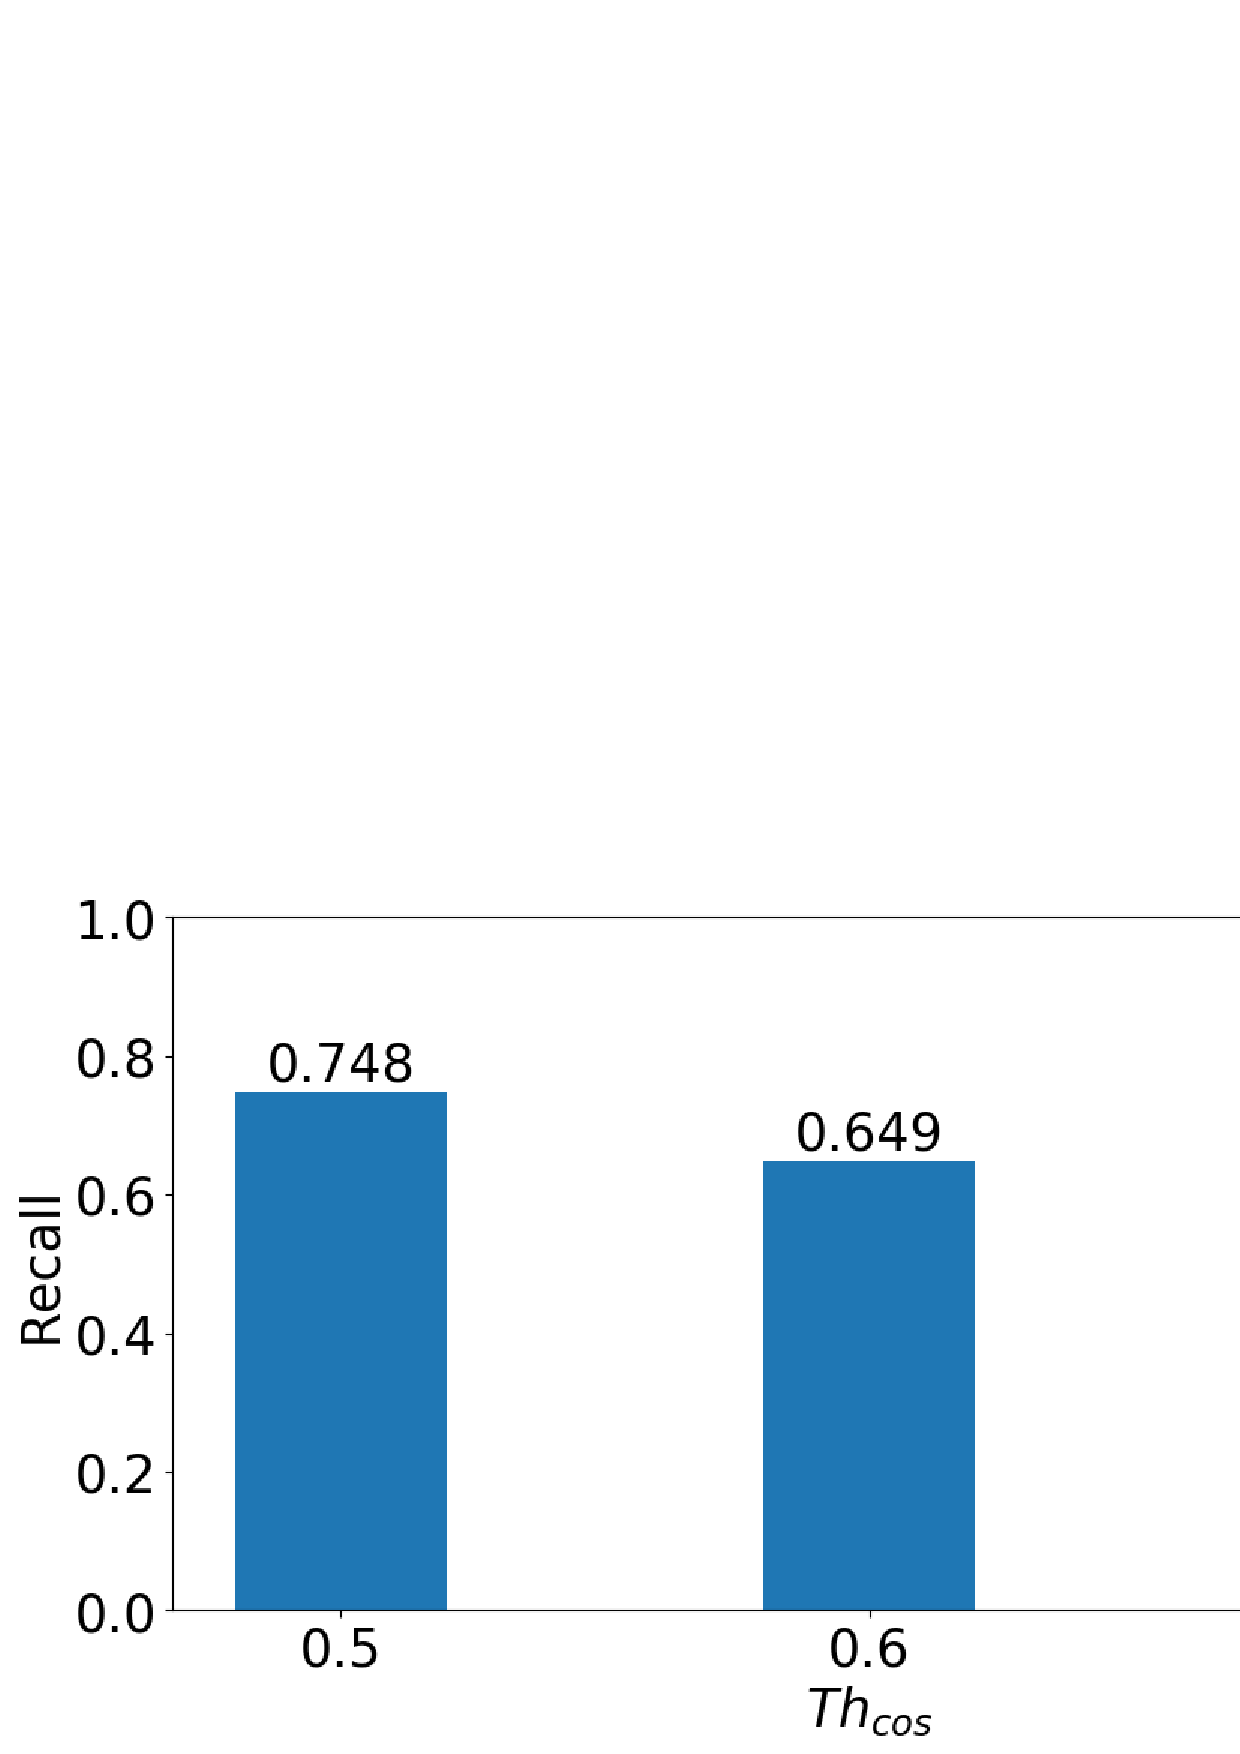
\includegraphics[keepaspectratio, scale=0.27]
                          {./figure/baseline_r.eps}}
      \end{minipage}

      \begin{minipage}{0.06\hsize}
        \hspace{2mm}
      \end{minipage}
 
%----- precision -----
 
      \begin{minipage}{0.47\hsize}
        \centering
          \subfigure[Precision]{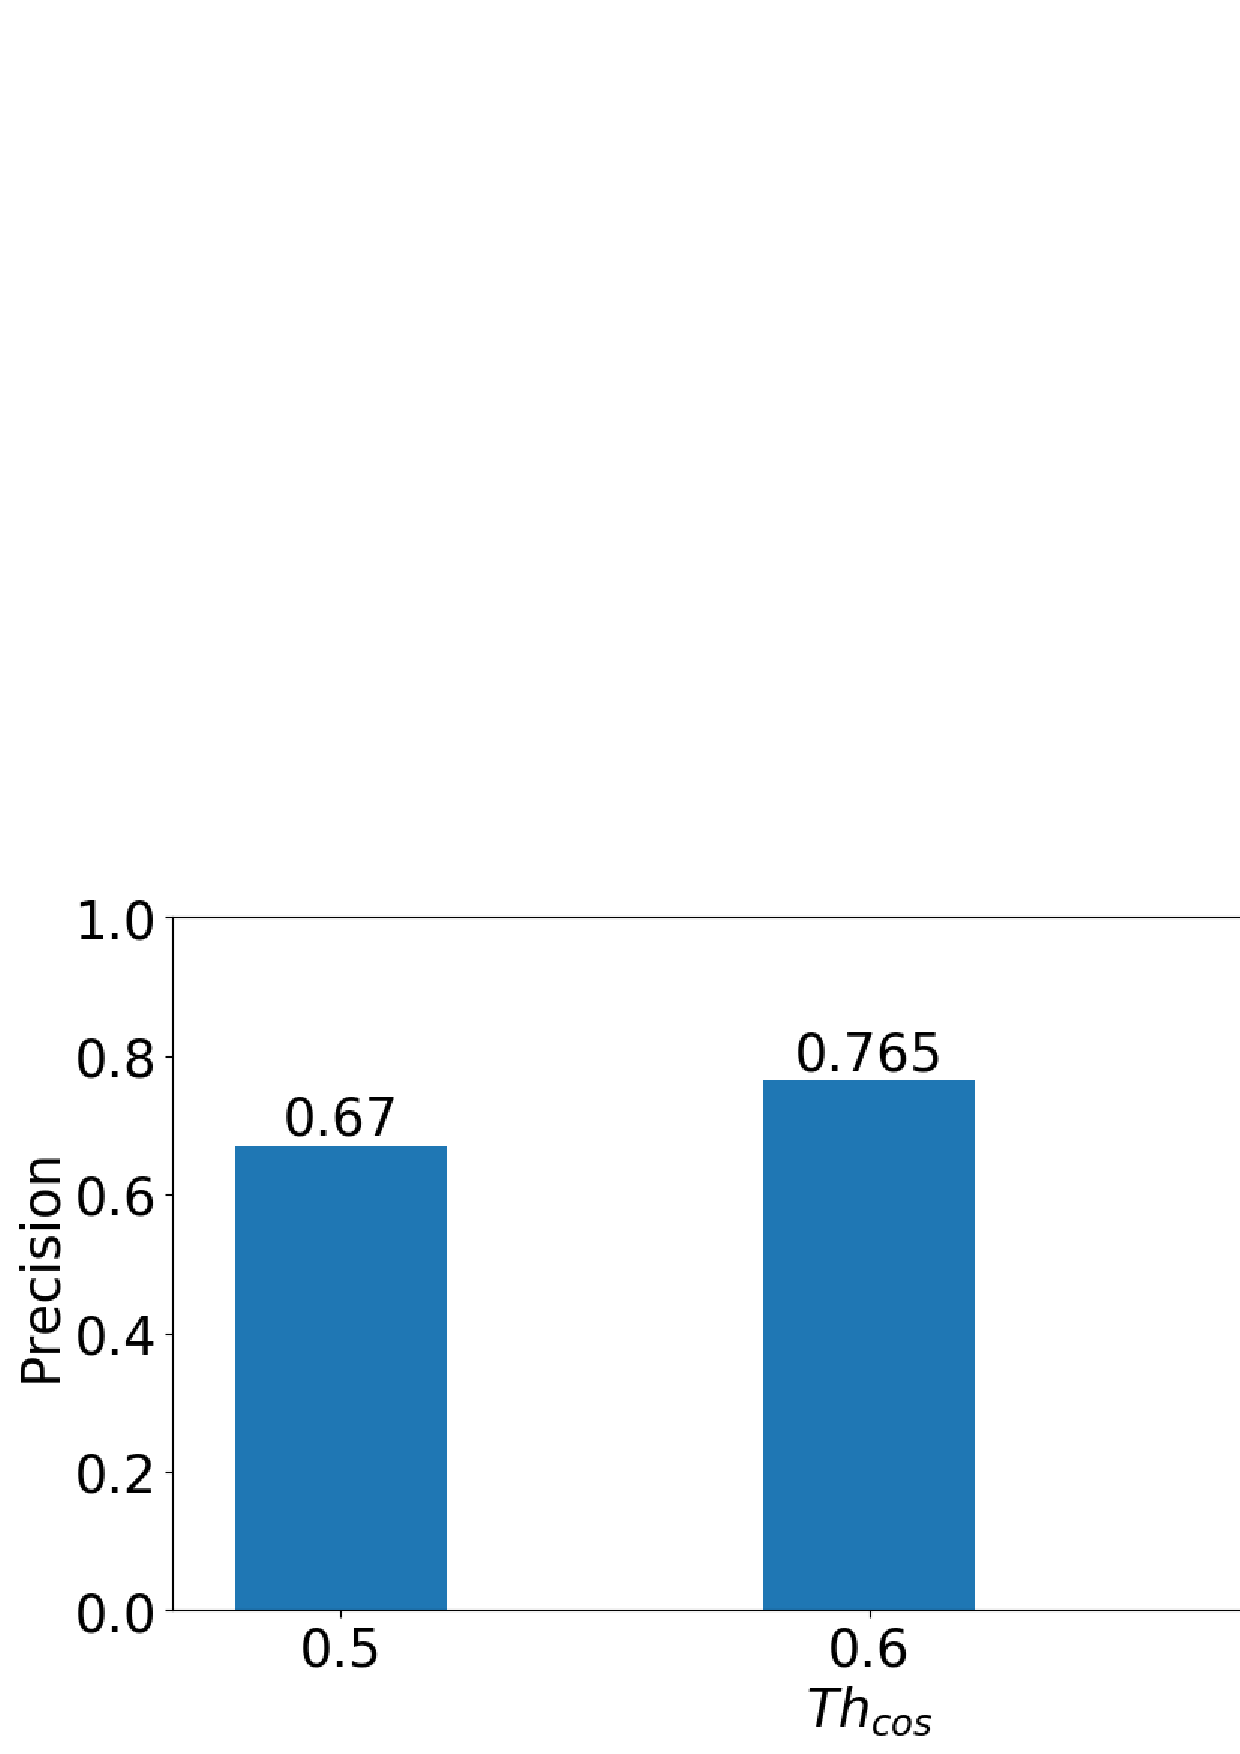
\includegraphics[keepaspectratio, scale=0.27]
                          {./figure/baseline_p.eps}}
      \end{minipage} \\

      \begin{minipage}{0.06\hsize}
        \vspace{10mm}
      \end{minipage} \\
 
 
%----- fmeasure -----
 
      \begin{minipage}{0.47\hsize}
        \centering
          \subfigure[F-measure]{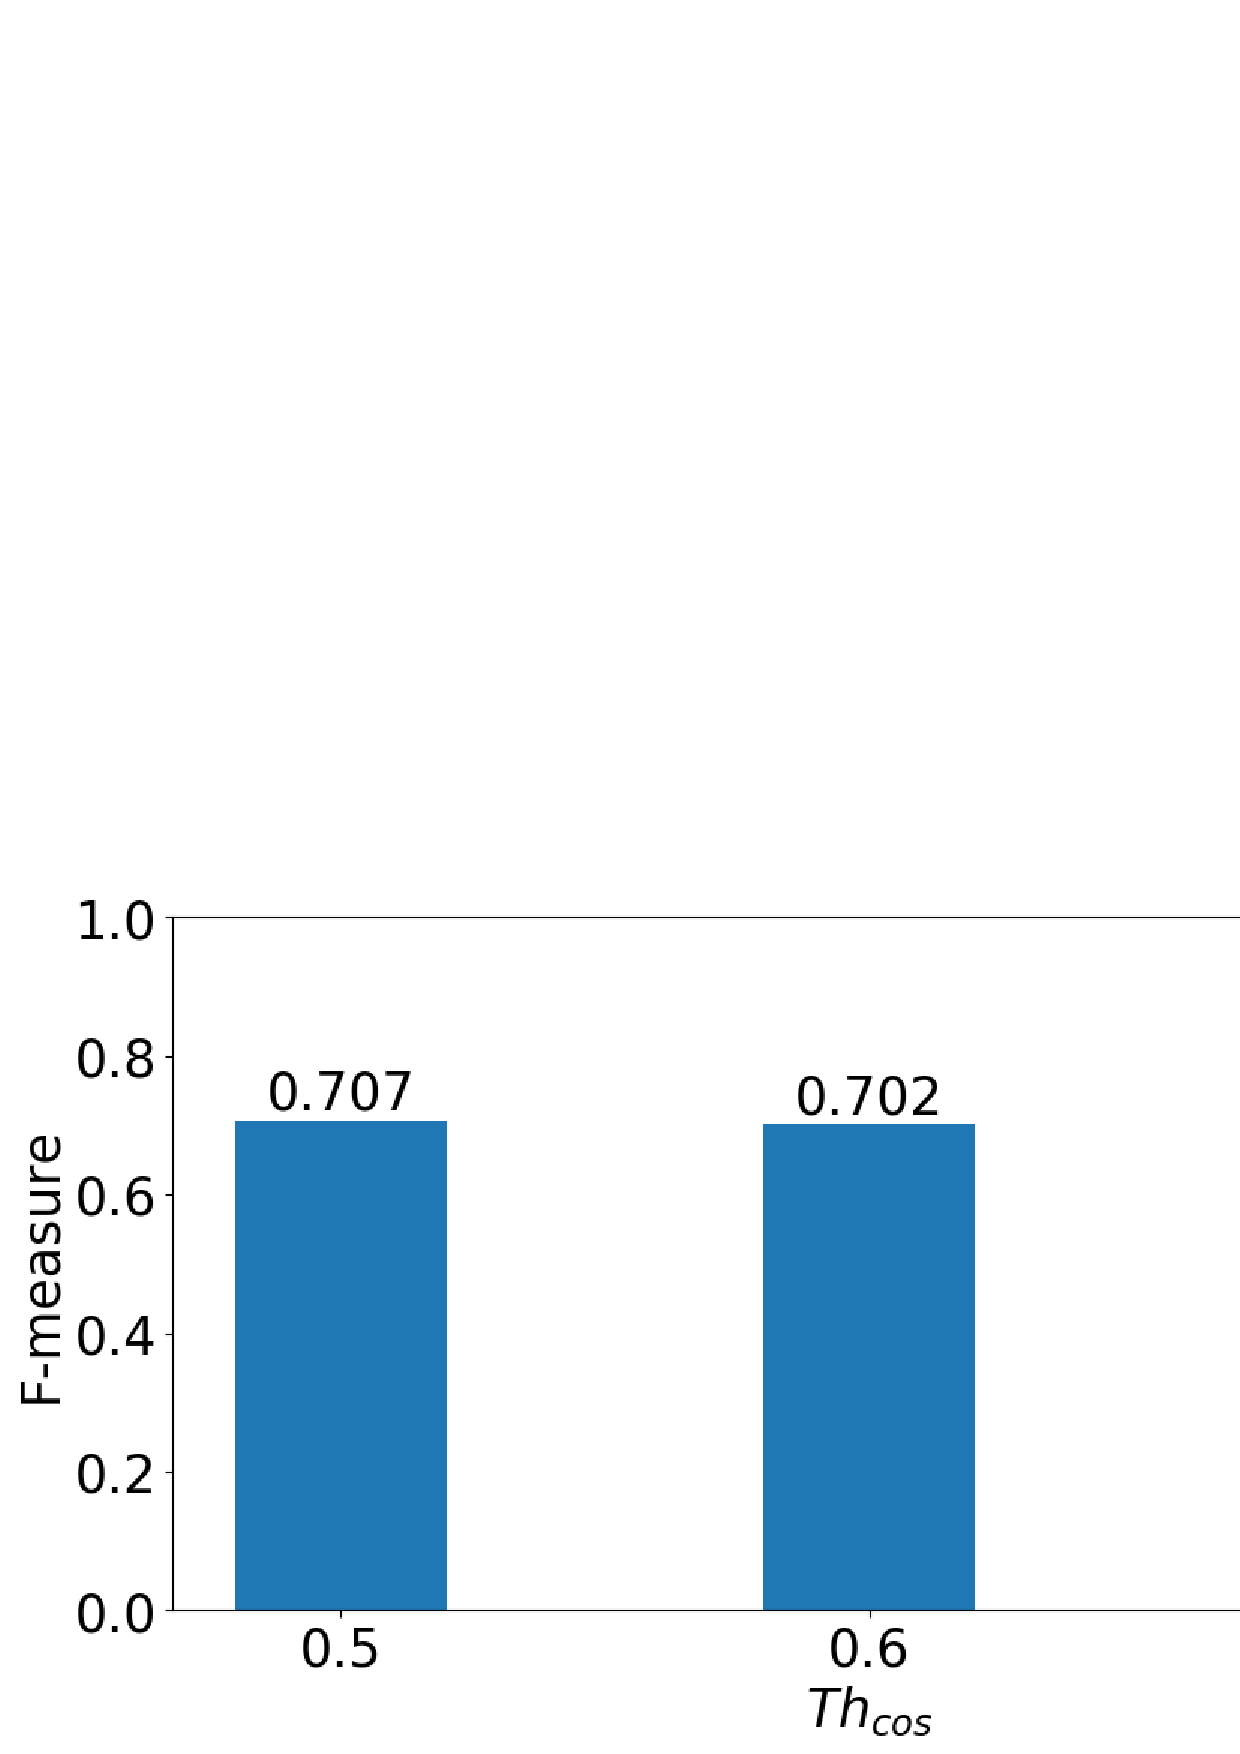
\includegraphics[keepaspectratio, scale=0.27]
                          {./figure/baseline_f.eps} \label{baseline_fmeasure}}
      \end{minipage}

      \begin{minipage}{0.06\hsize}
        \hspace{2mm}
      \end{minipage}
 
%----- acc time -----
 
      \begin{minipage}{0.47\hsize}
        \centering
          \subfigure[$Acc_{time}$]{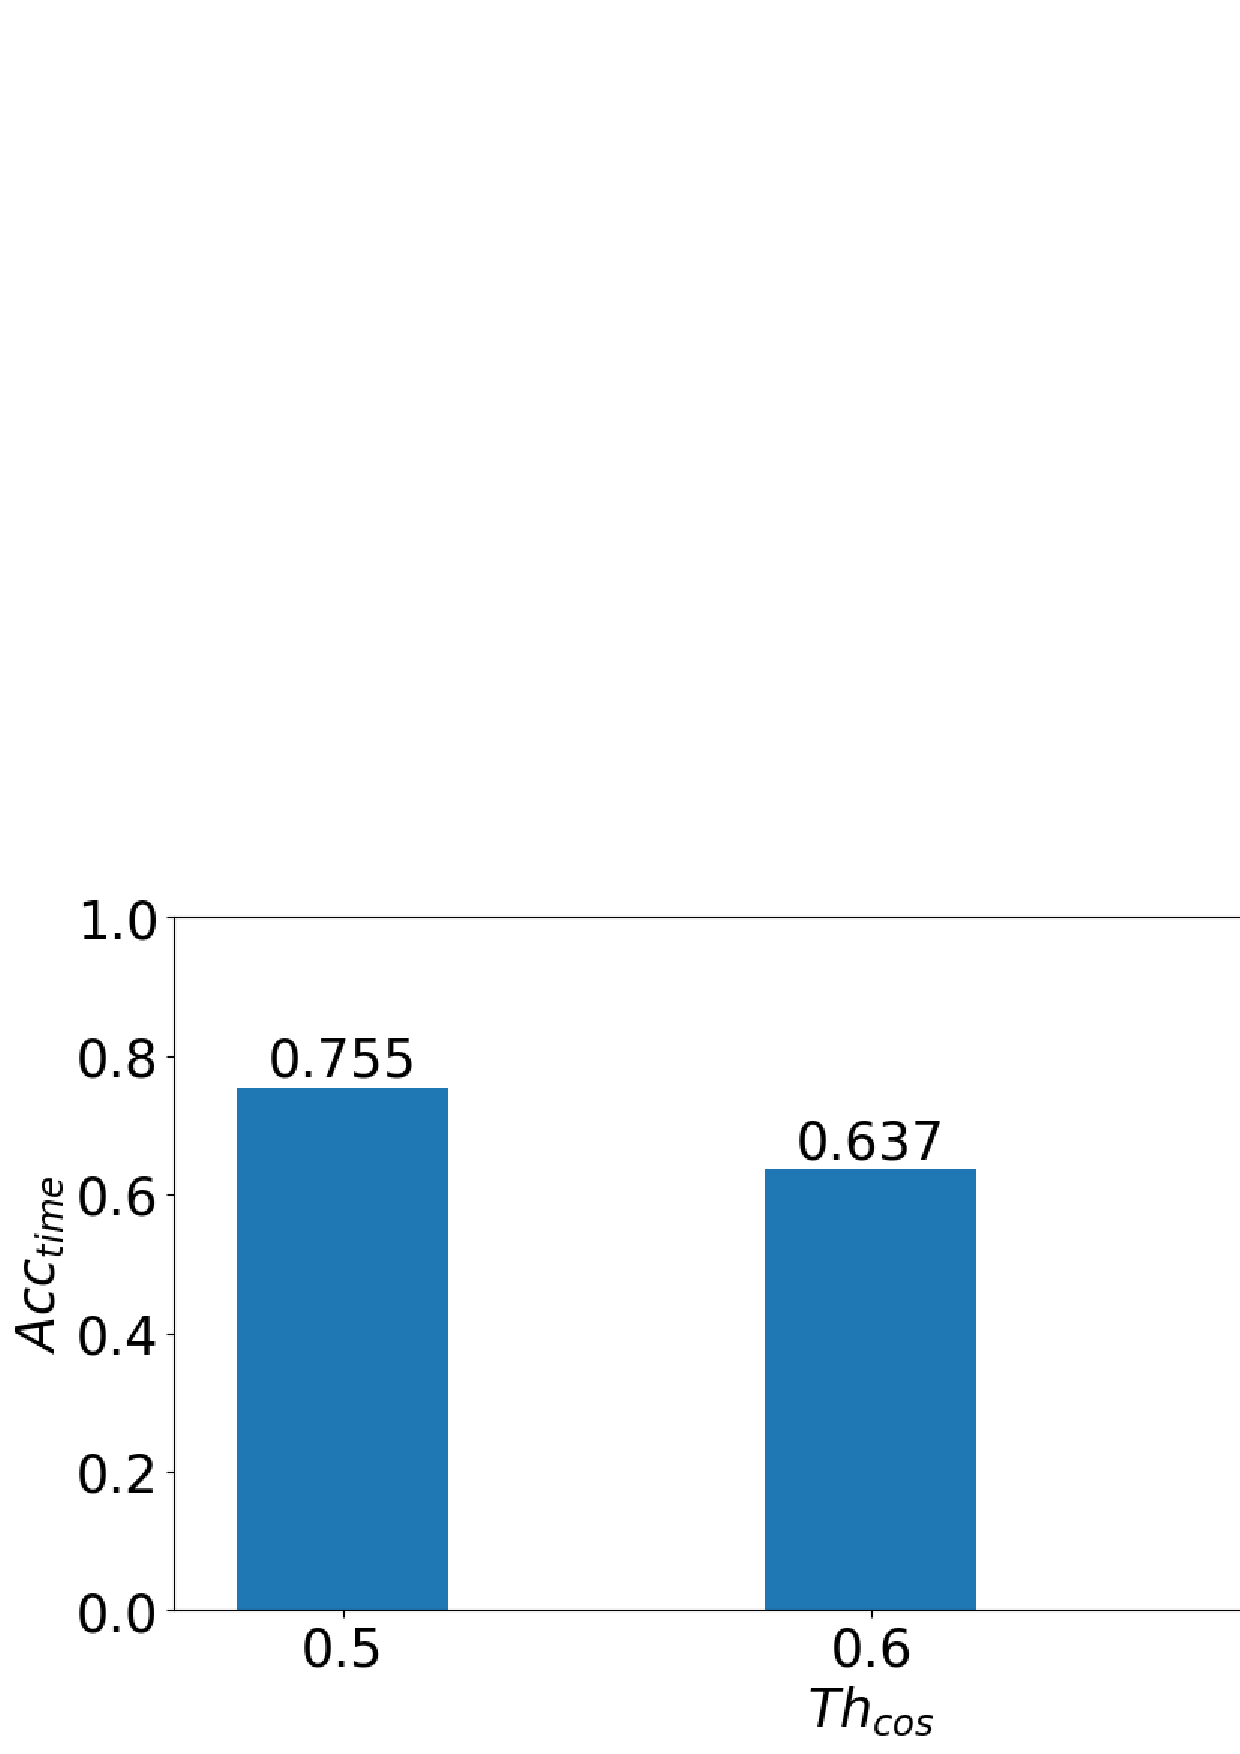
\includegraphics[keepaspectratio, scale=0.27]
                          {./figure/baseline_acc.eps}}
      \end{minipage}
    
    \end{tabular}
\caption{Baselineによる発話区間検出精度 \label{fig:result_anchor_baseline}}
\end{figure} 


\begin{table}[H]
  \begin{center}
    \caption{Baselineによる各ニュース番組音声のニュースアンカーの発話検出精度($Th_{cos}=0.5$) \label{table:baseline_eachnews}}
    \begin{tabular}{|c||c|c|c|c|} \hline
データID & Recall & Precision & F-meature & 作成したクラスタ数\\ \hline
ニュース1 & 0.970 & 0.623 & 0.758 & 1 \\ \hline
ニュース2 & 0.709 & 0.437 & 0.540 & 2 \\ \hline
ニュース3 & 0.736 & 0.719 & 0.727 & 2 \\ \hline
ニュース4 & 0.728 & 0.661 & 0.693 & 2 \\ \hline
ニュース5 & 0.683 & 0.947 & 0.793 & 2 \\ \hline
    \end{tabular}
  \end{center}
\end{table}

%手法1の図
\begin{figure}[H]
  \centering
    \begin{tabular}{c}
 
%----- recall -----
 
      \begin{minipage}{0.47\hsize}
        \centering
          \subfigure[Recall]{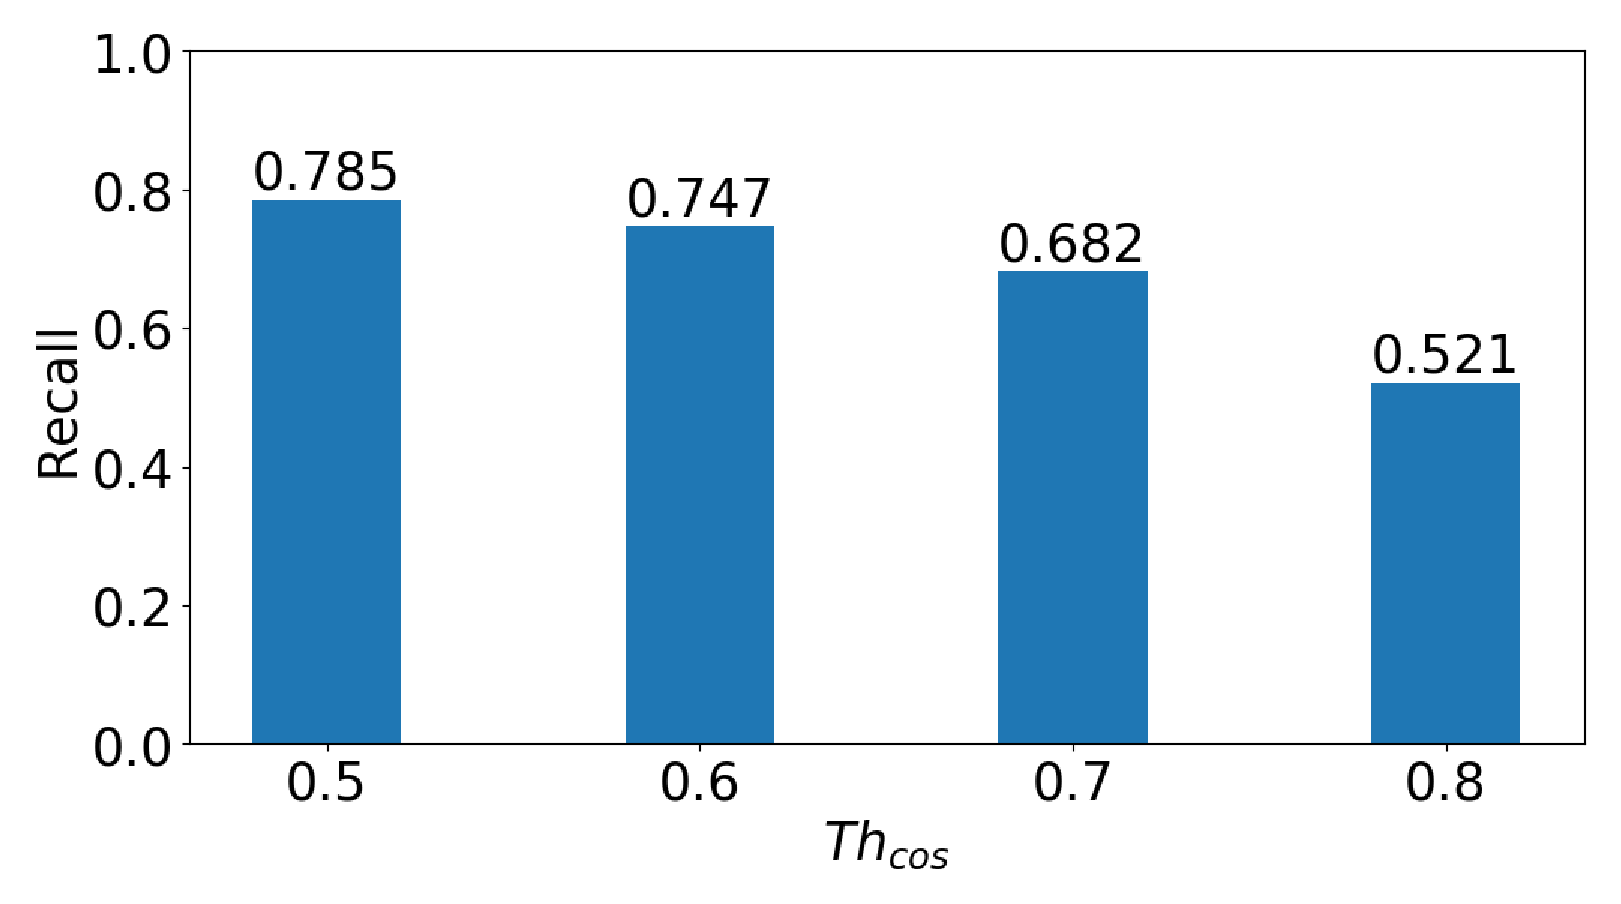
\includegraphics[keepaspectratio, scale=0.27]
                          {./figure/prob1_12_r.eps}}
      \end{minipage}

      \begin{minipage}{0.06\hsize}
        \hspace{2mm}
      \end{minipage}
 
%----- precision -----
 
      \begin{minipage}{0.47\hsize}
        \centering
          \subfigure[Precision]{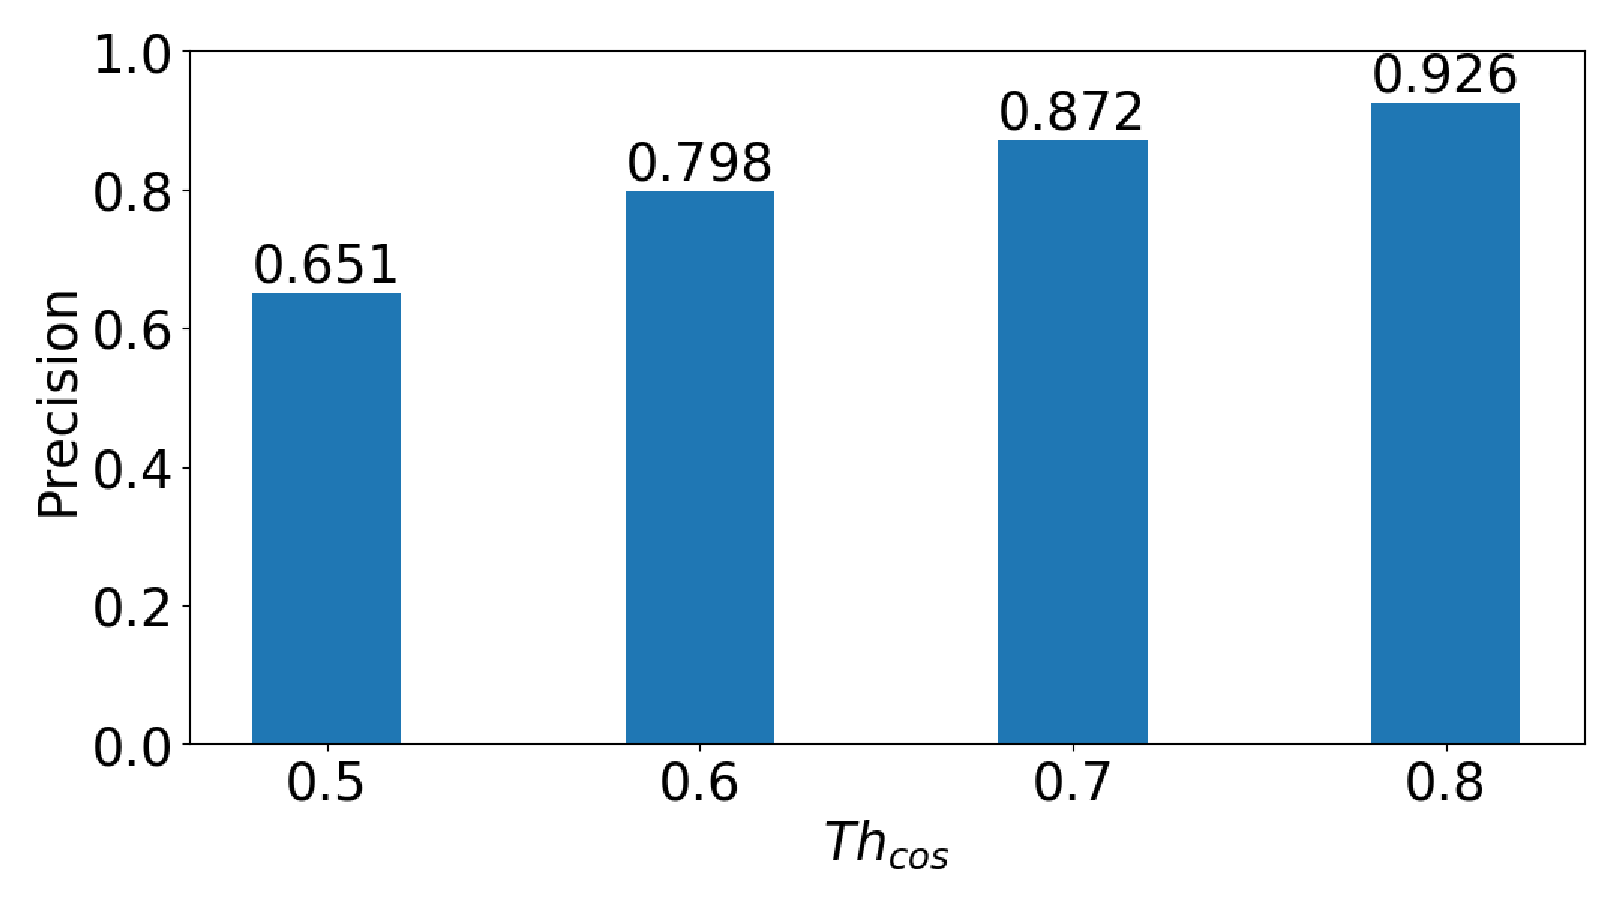
\includegraphics[keepaspectratio, scale=0.27]
                          {./figure/prob1_12_p.eps}}
      \end{minipage} \\

      \begin{minipage}{0.06\hsize}
        \vspace{10mm}
      \end{minipage} \\
 
 
%----- fmeasure -----
 
      \begin{minipage}{0.47\hsize}
        \centering
          \subfigure[F-measure]{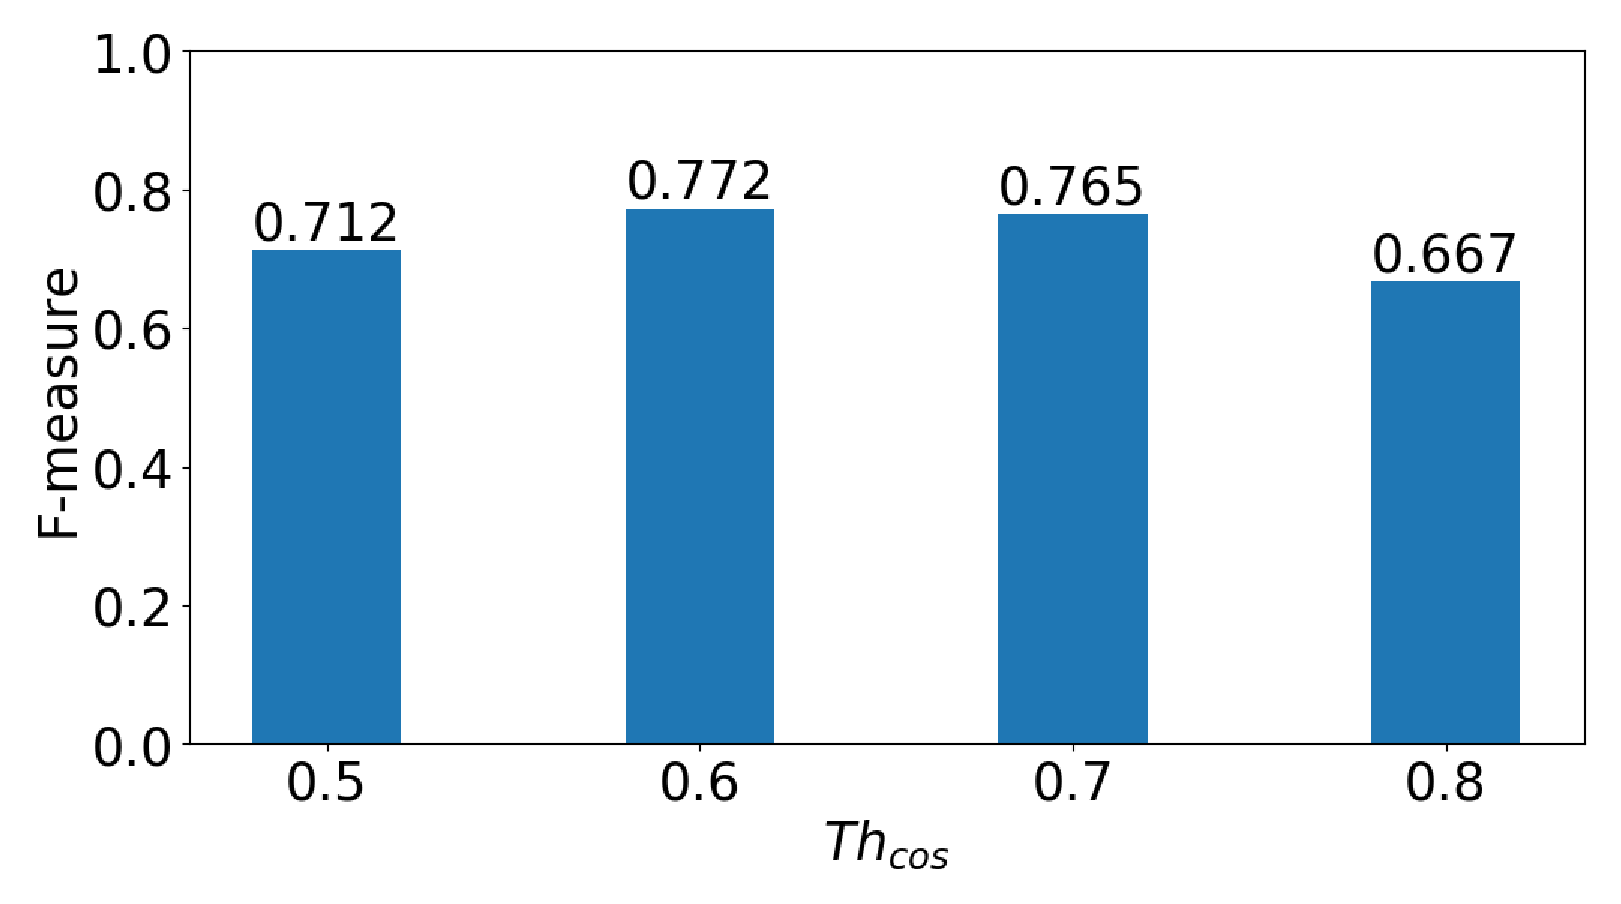
\includegraphics[keepaspectratio, scale=0.27]
                          {./figure/prob1_12_f.eps} \label{prob1_fmeasure}}
      \end{minipage}

      \begin{minipage}{0.06\hsize}
        \hspace{2mm}
      \end{minipage}
 
%----- acc time -----
 
      \begin{minipage}{0.47\hsize}
        \centering
          \subfigure[$Acc_{time}$]{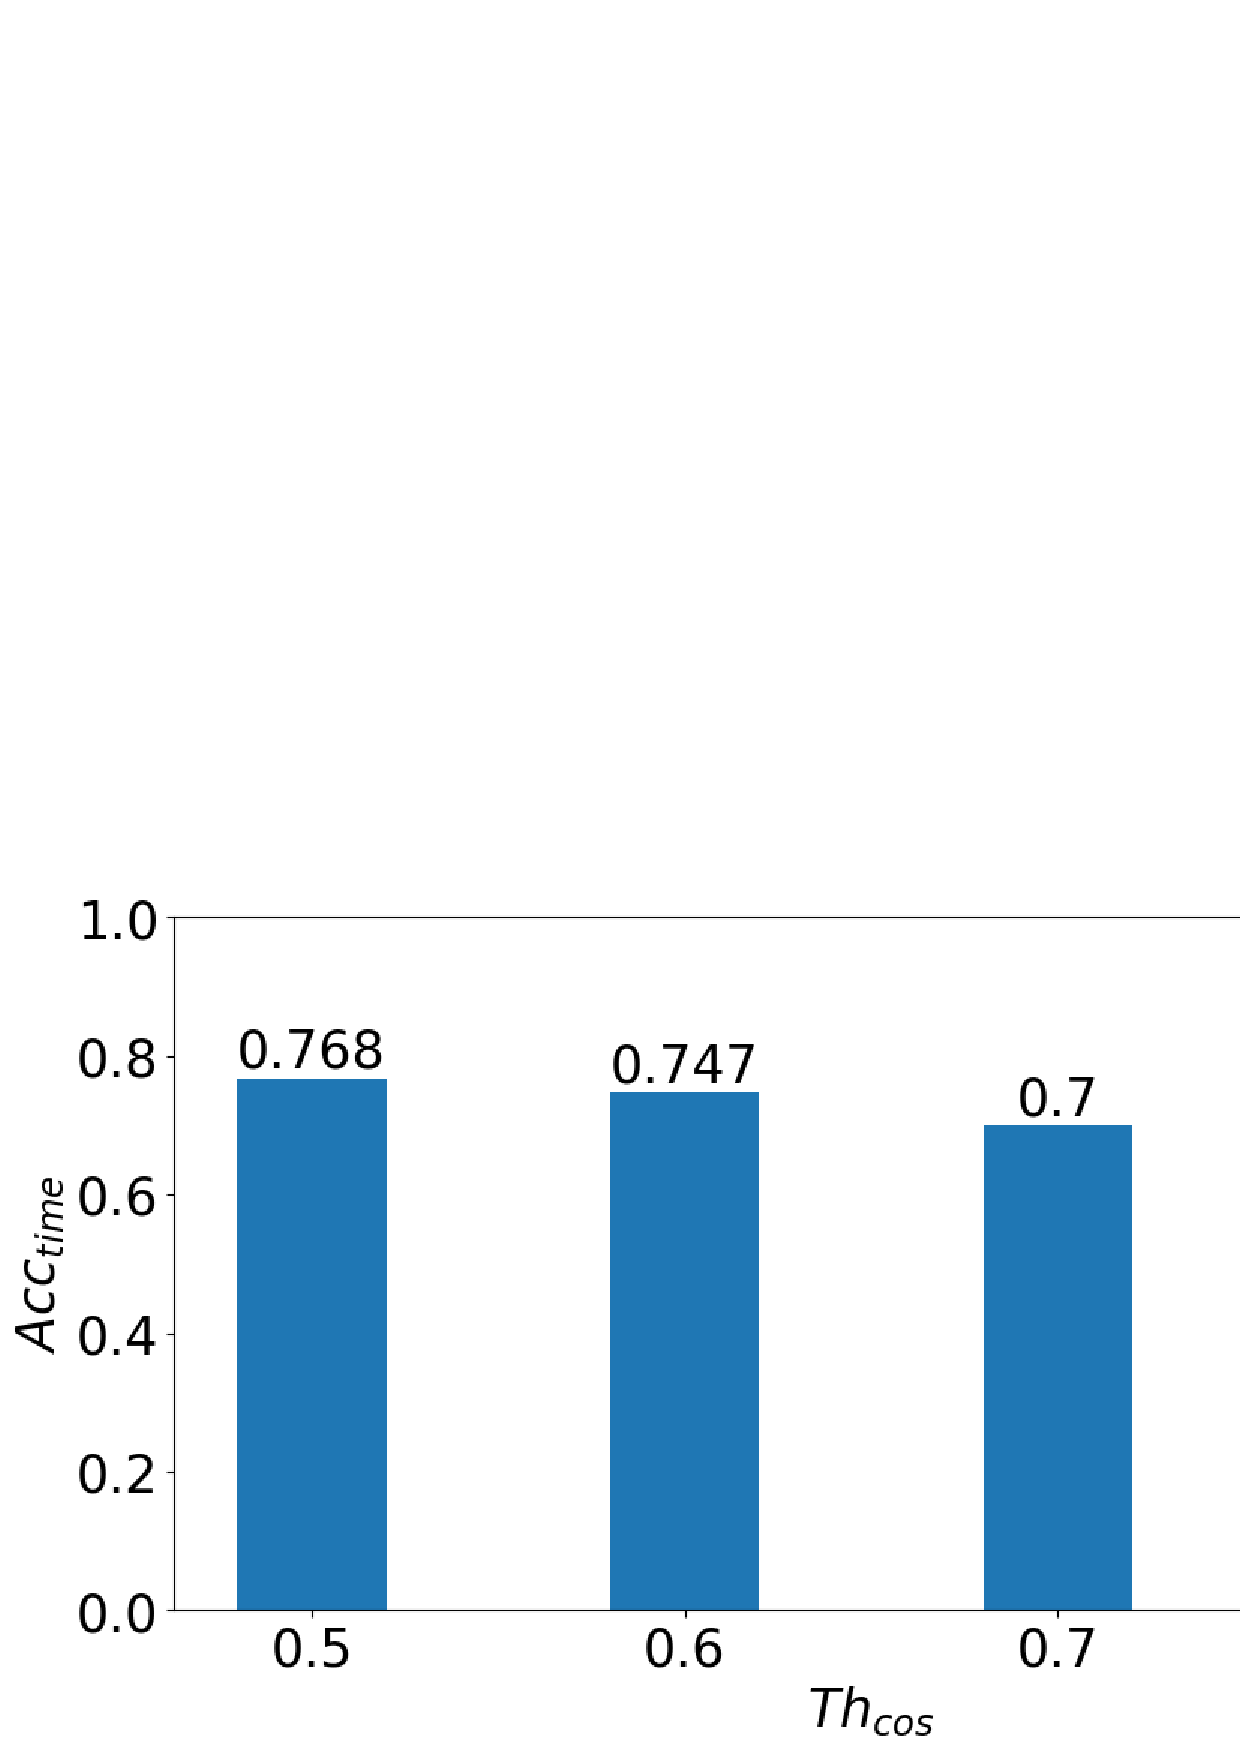
\includegraphics[keepaspectratio, scale=0.27]
                          {./figure/prob1_12_acc.eps}}
      \end{minipage}
    
    \end{tabular}
\caption{手法1によるアンカーの発話区間検出精度 ($Th_{time}=1.2$) \label{fig:result_anchor_prob1}}
\end{figure} 

\begin{table}[H]
  \begin{center}
    \caption{手法1による各ニュース番組音声のニュースアンカーの発話検出精度($Th_{cos}=0.6,Th_{time}=1.2$) }
    \begin{tabular}{|c||c|c|c|c|} \hline
データID & Recall & Precision & F-meature & 作成したクラスタ数\\ \hline
ニュース1 & 0.964 & 0.707 & 0.815 & 1 \\ \hline
ニュース2 & 0.764 & 0.685 & 0.722 & 2 \\ \hline
ニュース3 & 0.729 & 0.860 & 0.789 & 2 \\ \hline
ニュース4 & 0.683 & 0.741 & 0.711 & 2 \\ \hline
ニュース5 & 0.695 & 0.978 & 0.813 & 2 \\ \hline
    \end{tabular}
  \end{center}
\end{table}

%手法2の図
\begin{figure}[H]
  \centering
    \begin{tabular}{c}
 
%----- recall -----
 
      \begin{minipage}{0.47\hsize}
        \centering
          \subfigure[Recall]{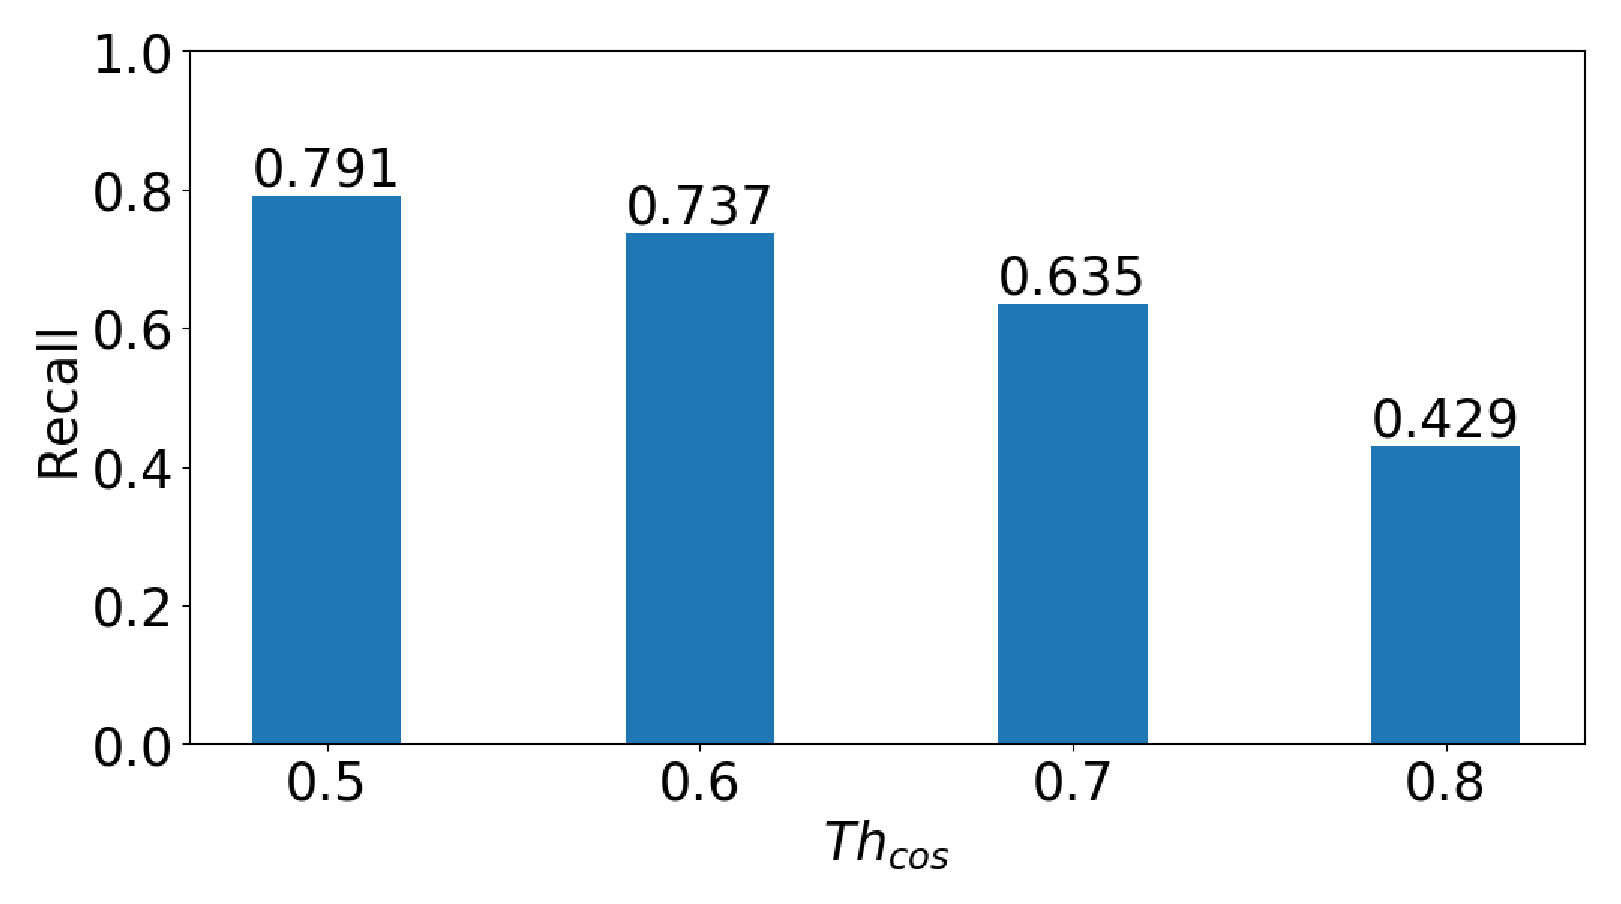
\includegraphics[keepaspectratio, scale=0.27]
                          {./figure/prob2_r.eps}}
      \end{minipage}

      \begin{minipage}{0.06\hsize}
        \hspace{2mm}
      \end{minipage}
 
%----- precision -----
 
      \begin{minipage}{0.47\hsize}
        \centering
          \subfigure[Precision]{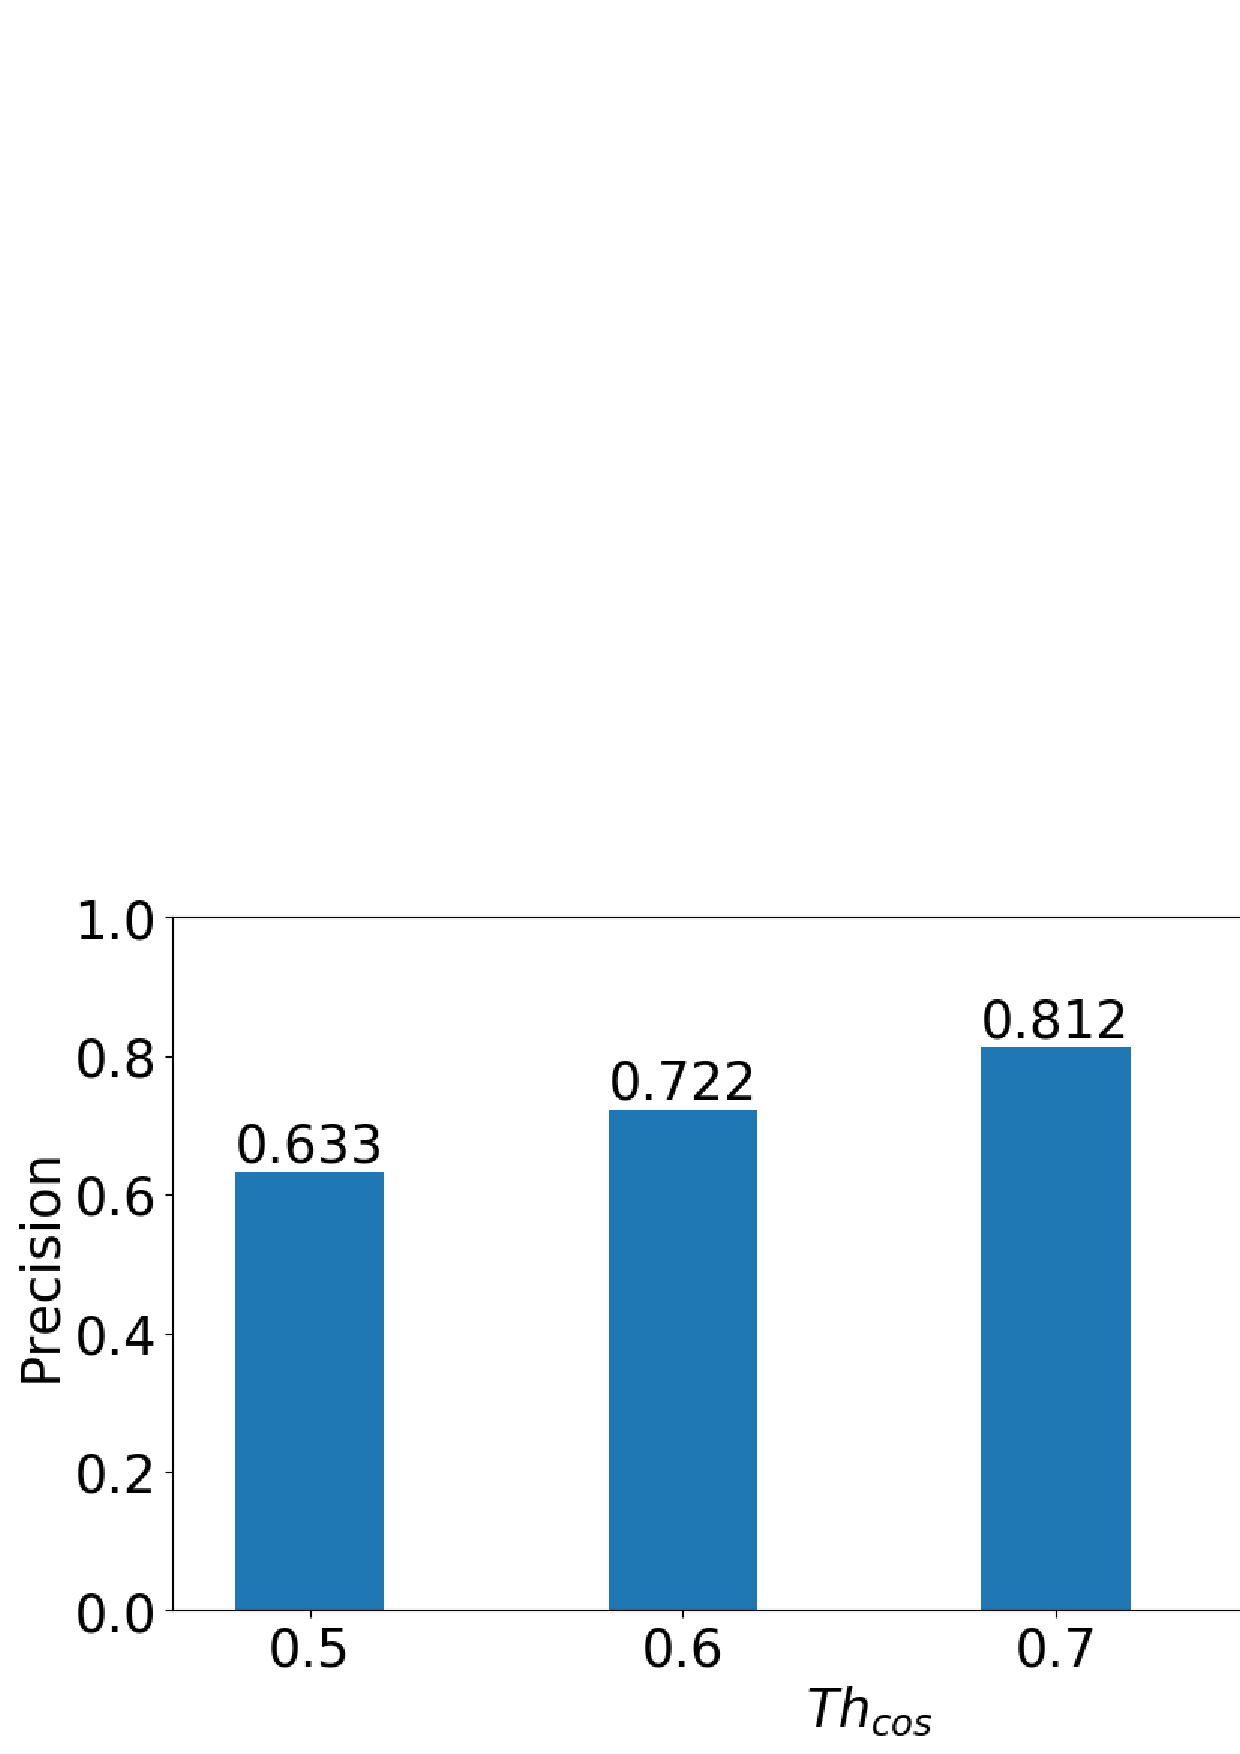
\includegraphics[keepaspectratio, scale=0.27]
                          {./figure/prob2_p.eps}}
      \end{minipage} \\

      \begin{minipage}{0.06\hsize}
        \vspace{10mm}
      \end{minipage} \\
 
 
%----- fmeasure -----
 
      \begin{minipage}{0.47\hsize}
        \centering
          \subfigure[F-measure]{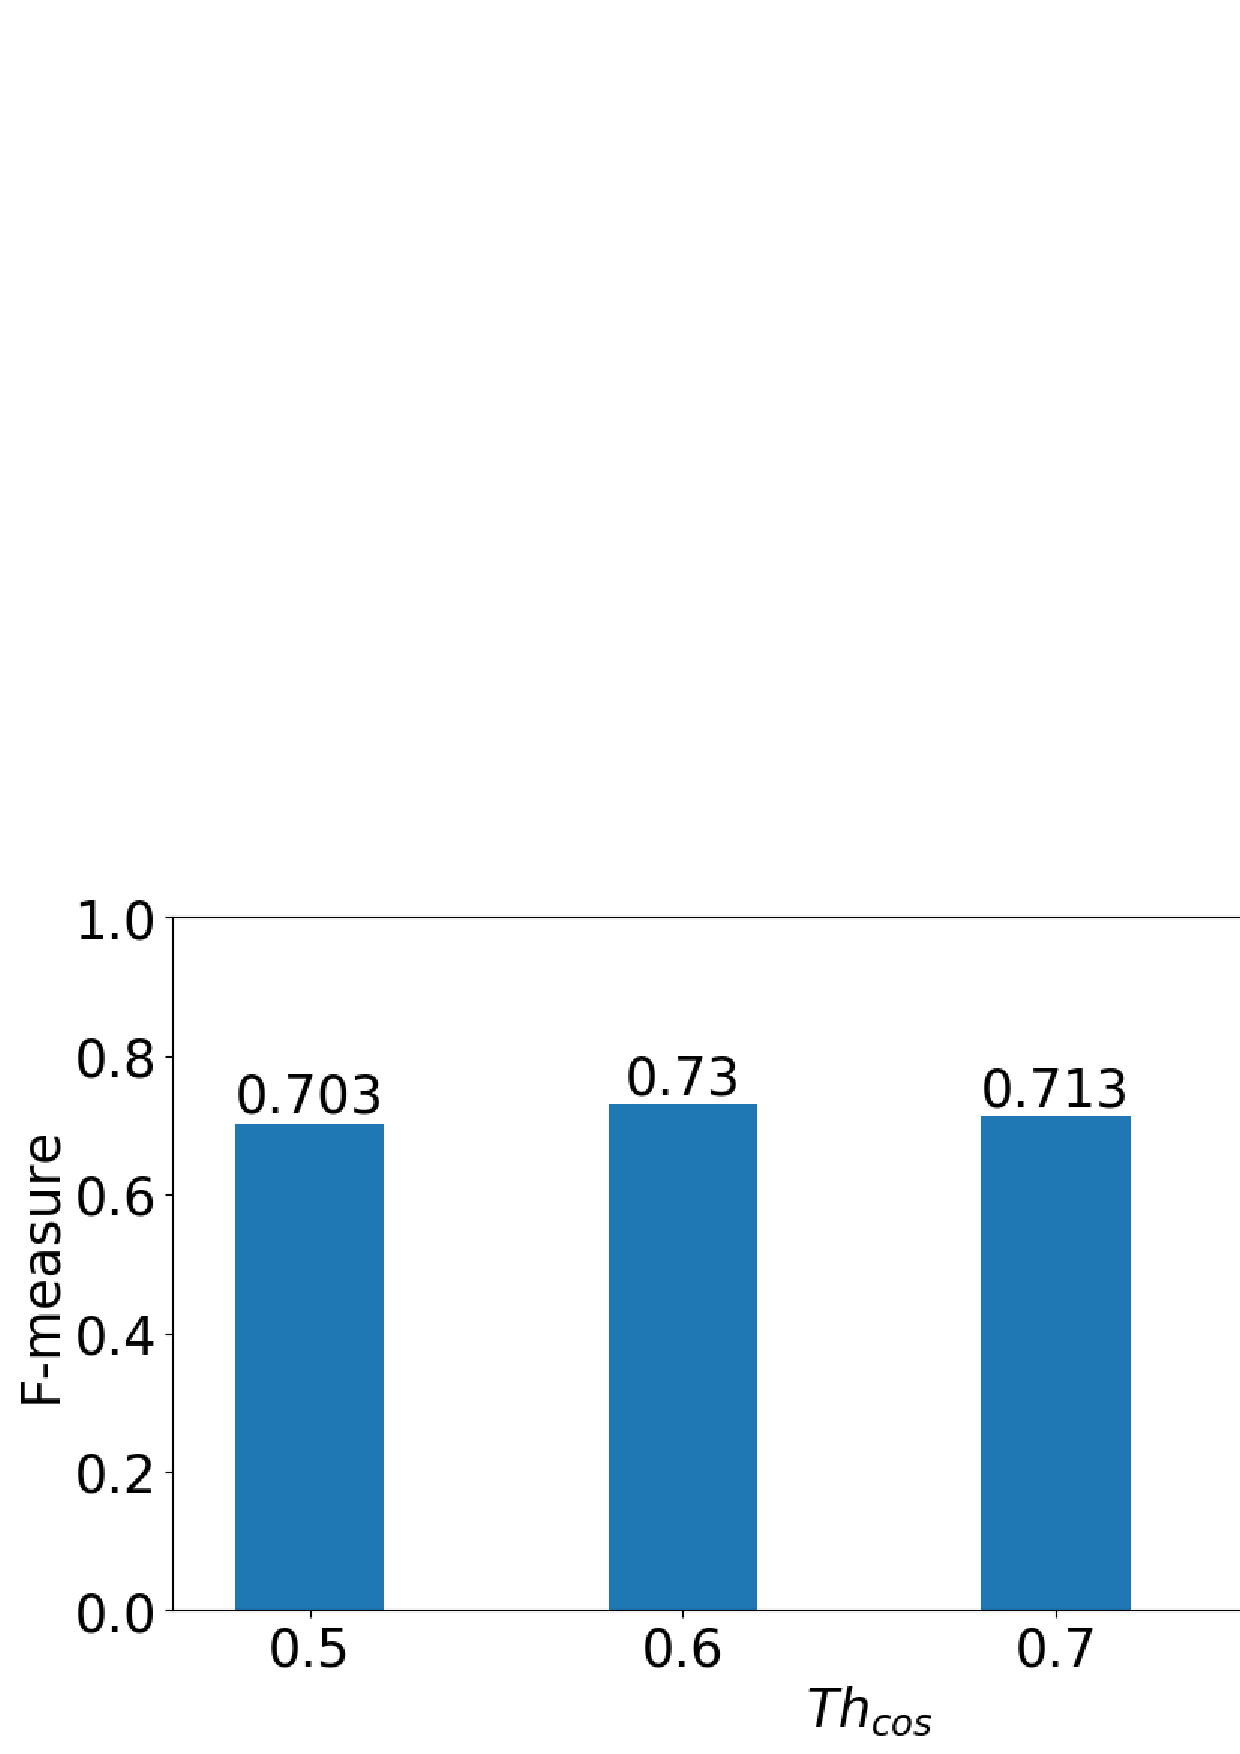
\includegraphics[keepaspectratio, scale=0.27]
                          {./figure/prob2_f.eps} \label{prob2_fmeasure}}
      \end{minipage}

      \begin{minipage}{0.06\hsize}
        \hspace{2mm}
      \end{minipage}
 
%----- acc time -----
 
      \begin{minipage}{0.47\hsize}
        \centering
          \subfigure[$Acc_{time}$]{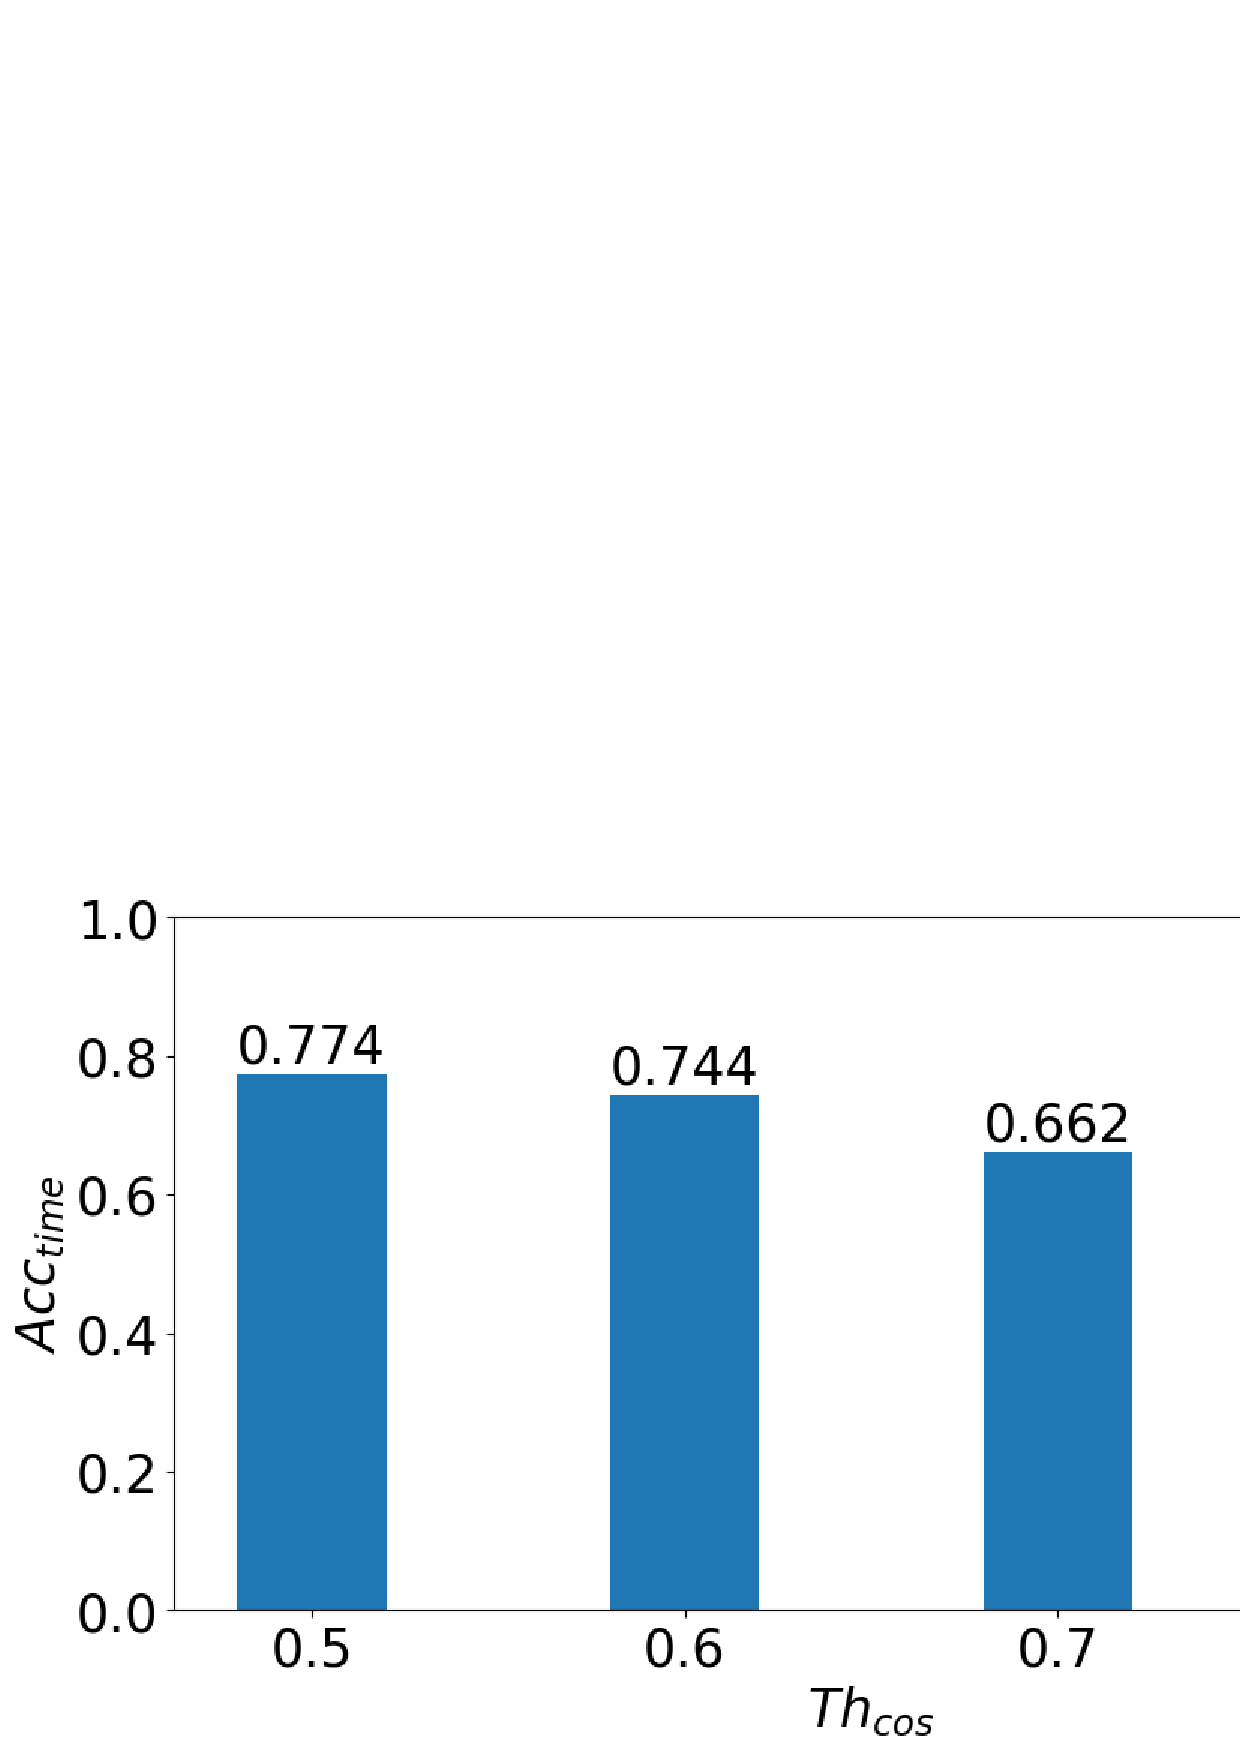
\includegraphics[keepaspectratio, scale=0.27]
                          {./figure/prob2_acc.eps}}
      \end{minipage}
    \end{tabular}
\caption{手法2によるニュースアンカーの発話検出精度 \label{fig:result_anchor_prob2}}
\end{figure} 

\begin{table}[H]
  \begin{center}
    \caption{手法2による各ニュース番組音声のニュースアンカーの発話検出精度($Th_{cos}=0.6$) }
    \begin{tabular}{|c||c|c|c|c|} \hline
データID & Recall & Precision & F-meature & 作成したクラスタ数\\ \hline
ニュース1 & 0.958 & 0.617 & 0.751 & 1 \\ \hline
ニュース2 & 0.788 & 0.512 & 0.621 & 2 \\ \hline
ニュース3 & 0.695 & 0.823 & 0.754 & 2 \\ \hline
ニュース4 & 0.683 & 0.732 & 0.707 & 2 \\ \hline
ニュース5 & 0.679 & 0.960 & 0.796 & 2 \\ \hline
    \end{tabular}
  \end{center}
\end{table}

%手法3の図
\begin{figure}[H]
  \centering
    \begin{tabular}{c}
 
%----- recall -----
 
      \begin{minipage}{0.47\hsize}
        \centering
          \subfigure[Recall]{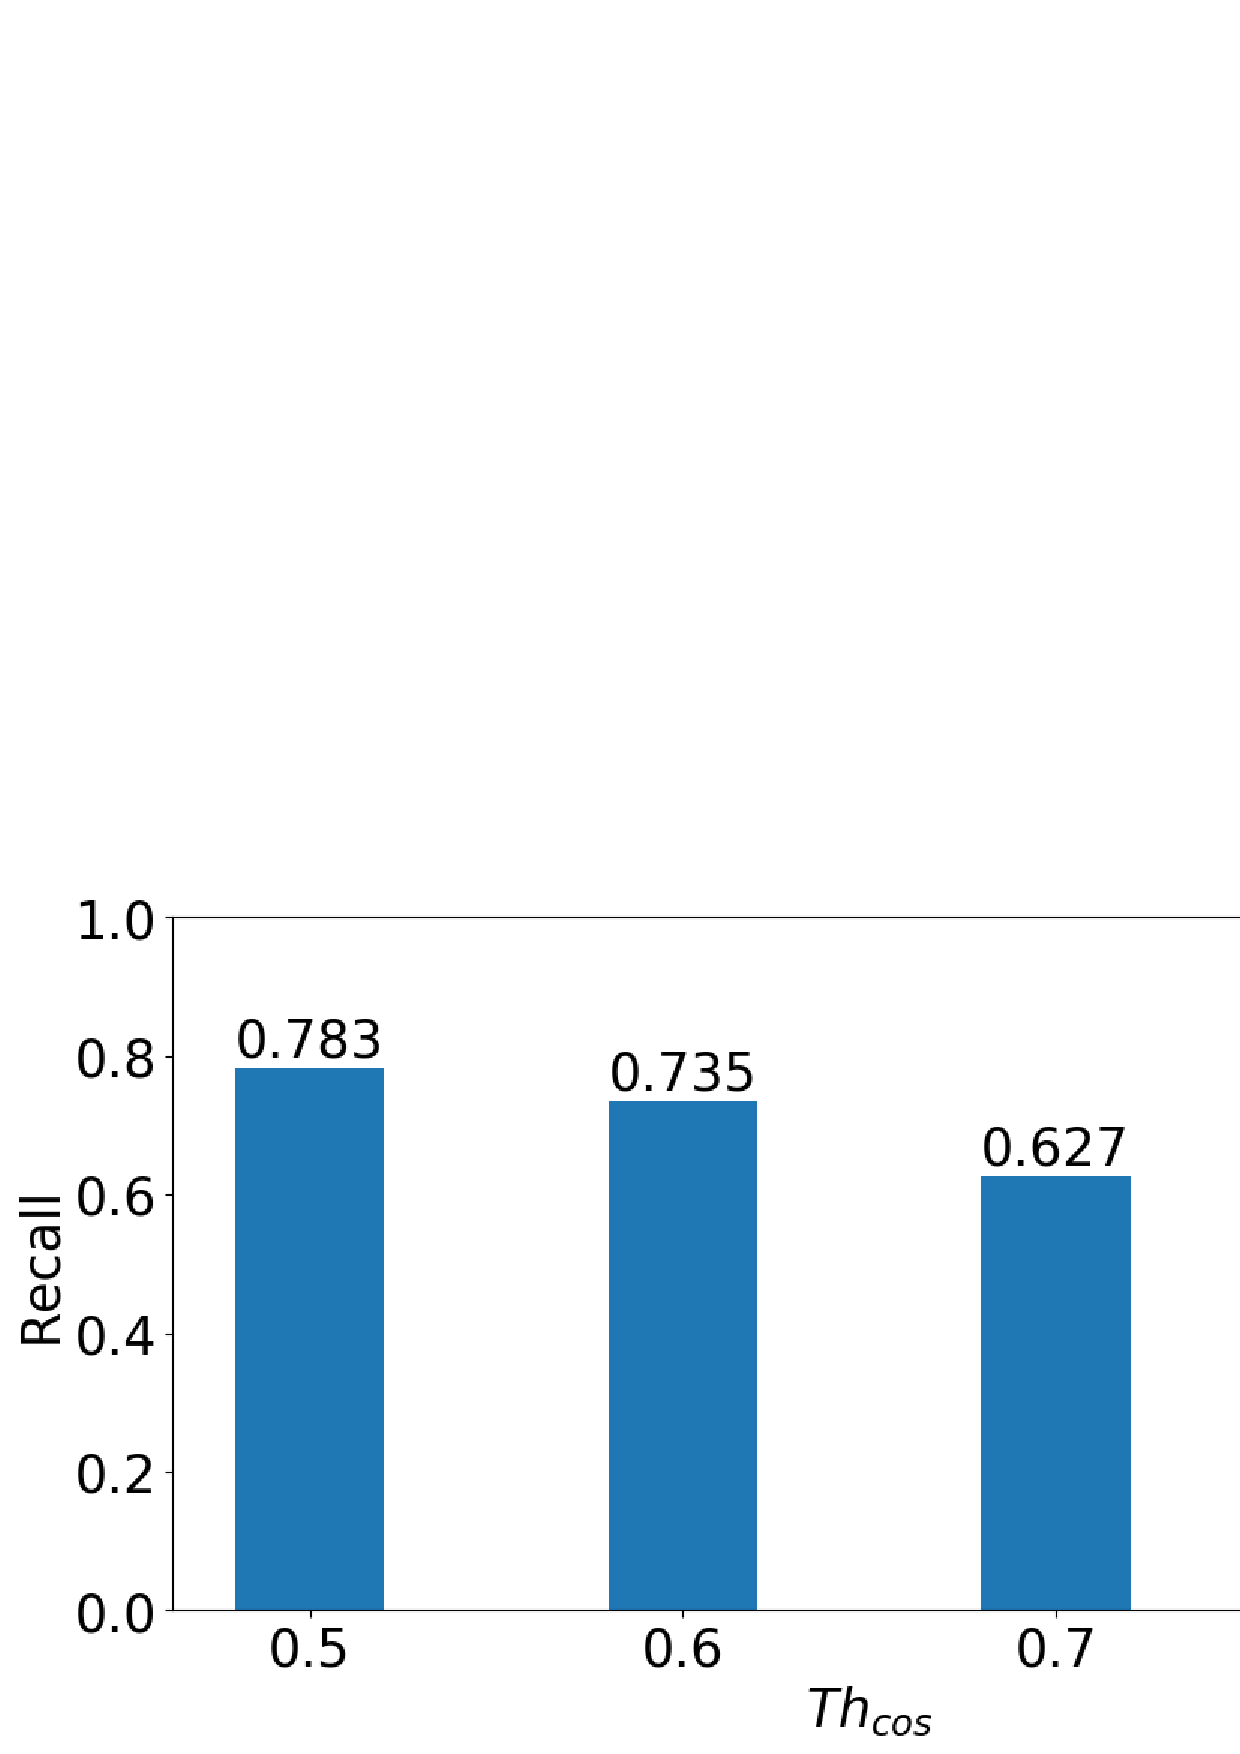
\includegraphics[keepaspectratio, scale=0.27]
                          {./figure/prob3_13_r.eps}}
      \end{minipage}

      \begin{minipage}{0.06\hsize}
        \hspace{2mm}
      \end{minipage}
 
%----- precision -----
 
      \begin{minipage}{0.47\hsize}
        \centering
          \subfigure[Precision]{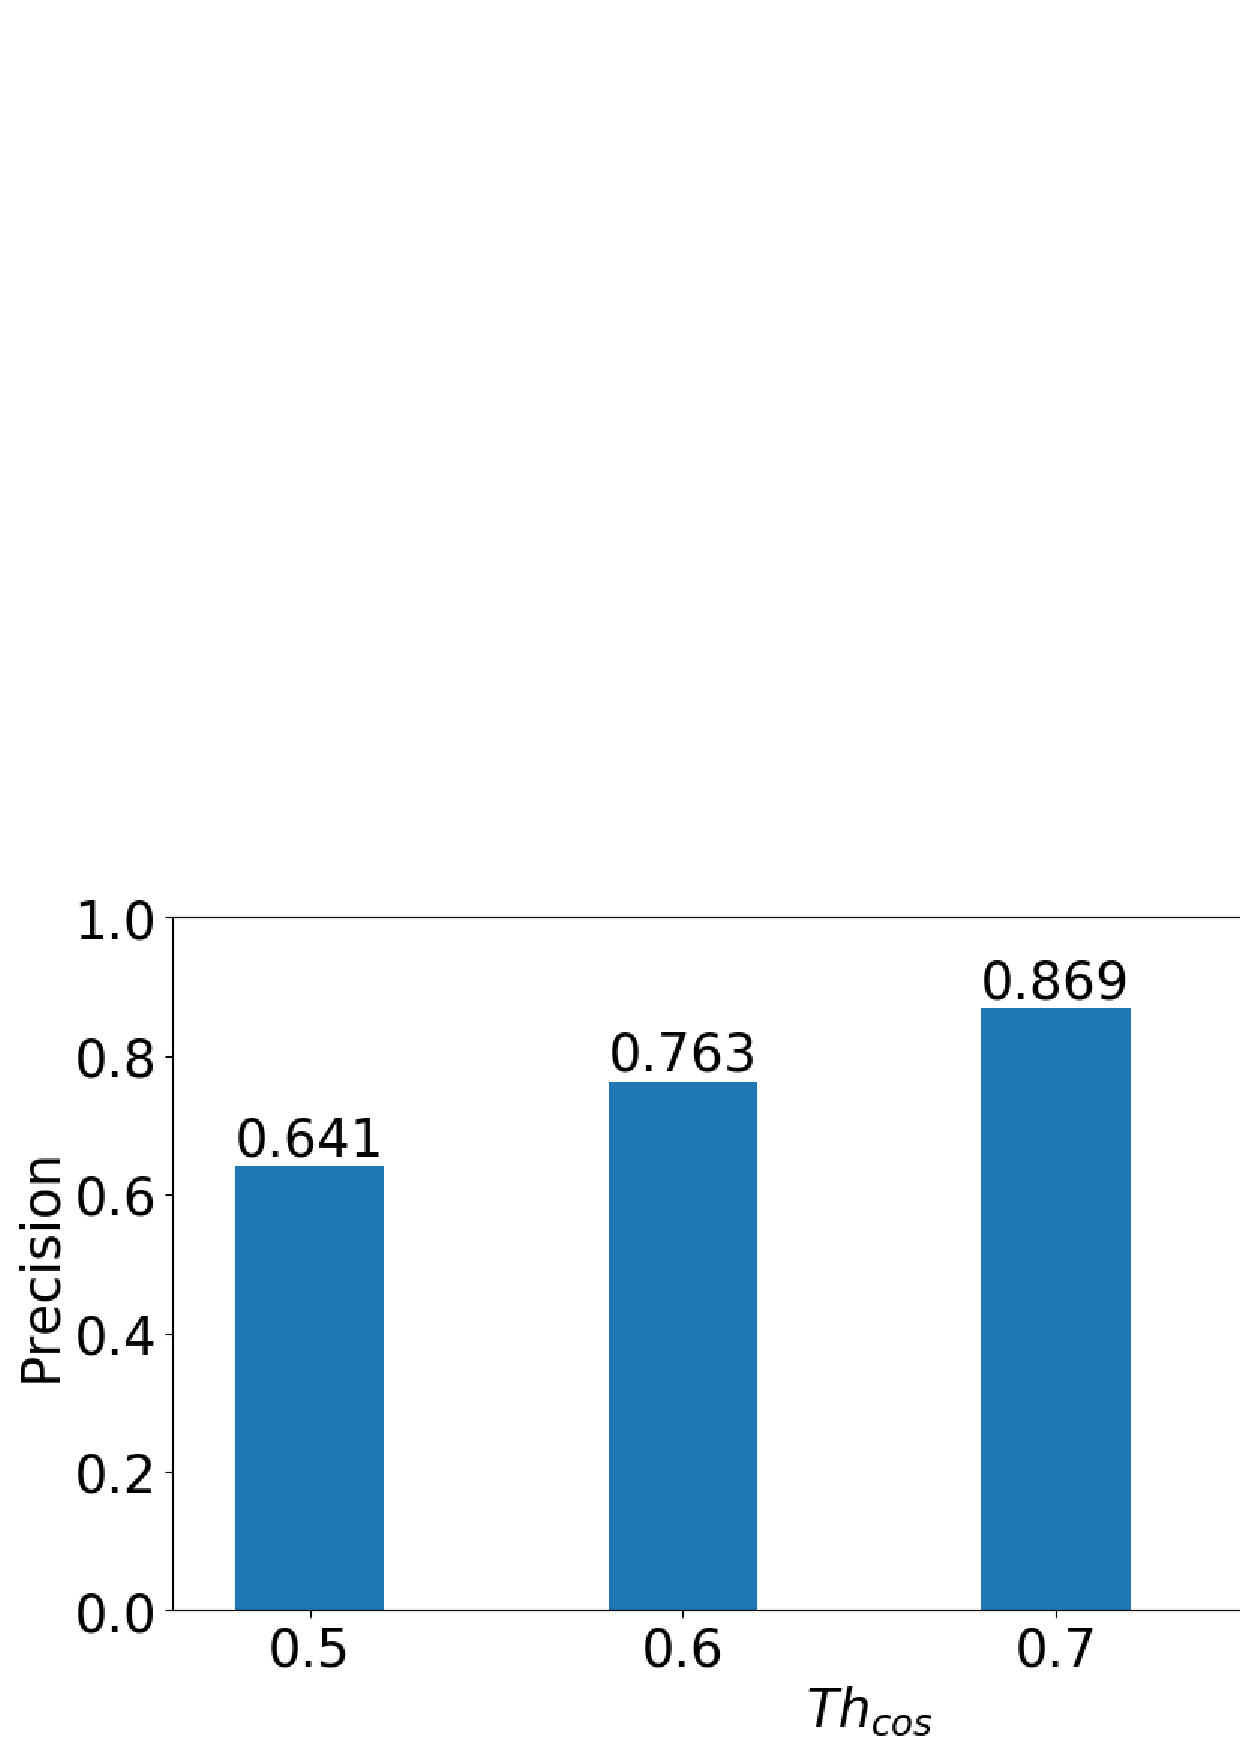
\includegraphics[keepaspectratio, scale=0.27]
                          {./figure/prob3_13_p.eps}}
      \end{minipage} \\

      \begin{minipage}{0.06\hsize}
        \vspace{10mm}
      \end{minipage} \\
 
 
%----- fmeasure -----
 
      \begin{minipage}{0.47\hsize}
        \centering
          \subfigure[F-measure]{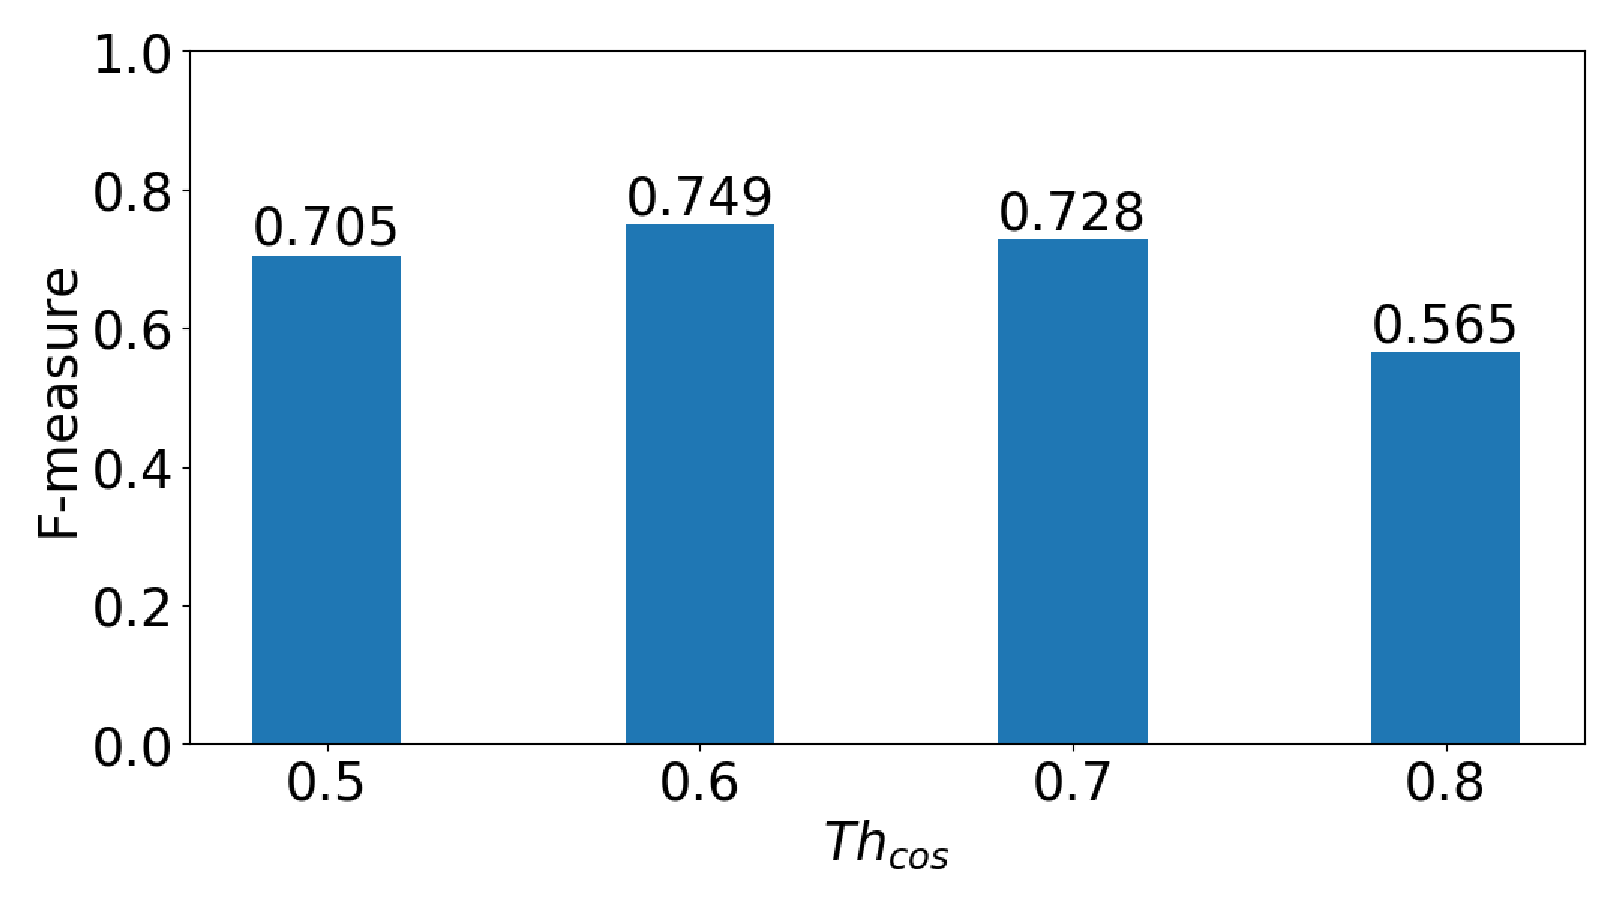
\includegraphics[keepaspectratio, scale=0.27]
                          {./figure/prob3_13_f.eps} \label{prob3_fmeasure}}
      \end{minipage}

      \begin{minipage}{0.06\hsize}
        \hspace{2mm}
      \end{minipage}
 
%----- acc time -----
 
      \begin{minipage}{0.47\hsize}
        \centering
          \subfigure[$Acc_{time}$]{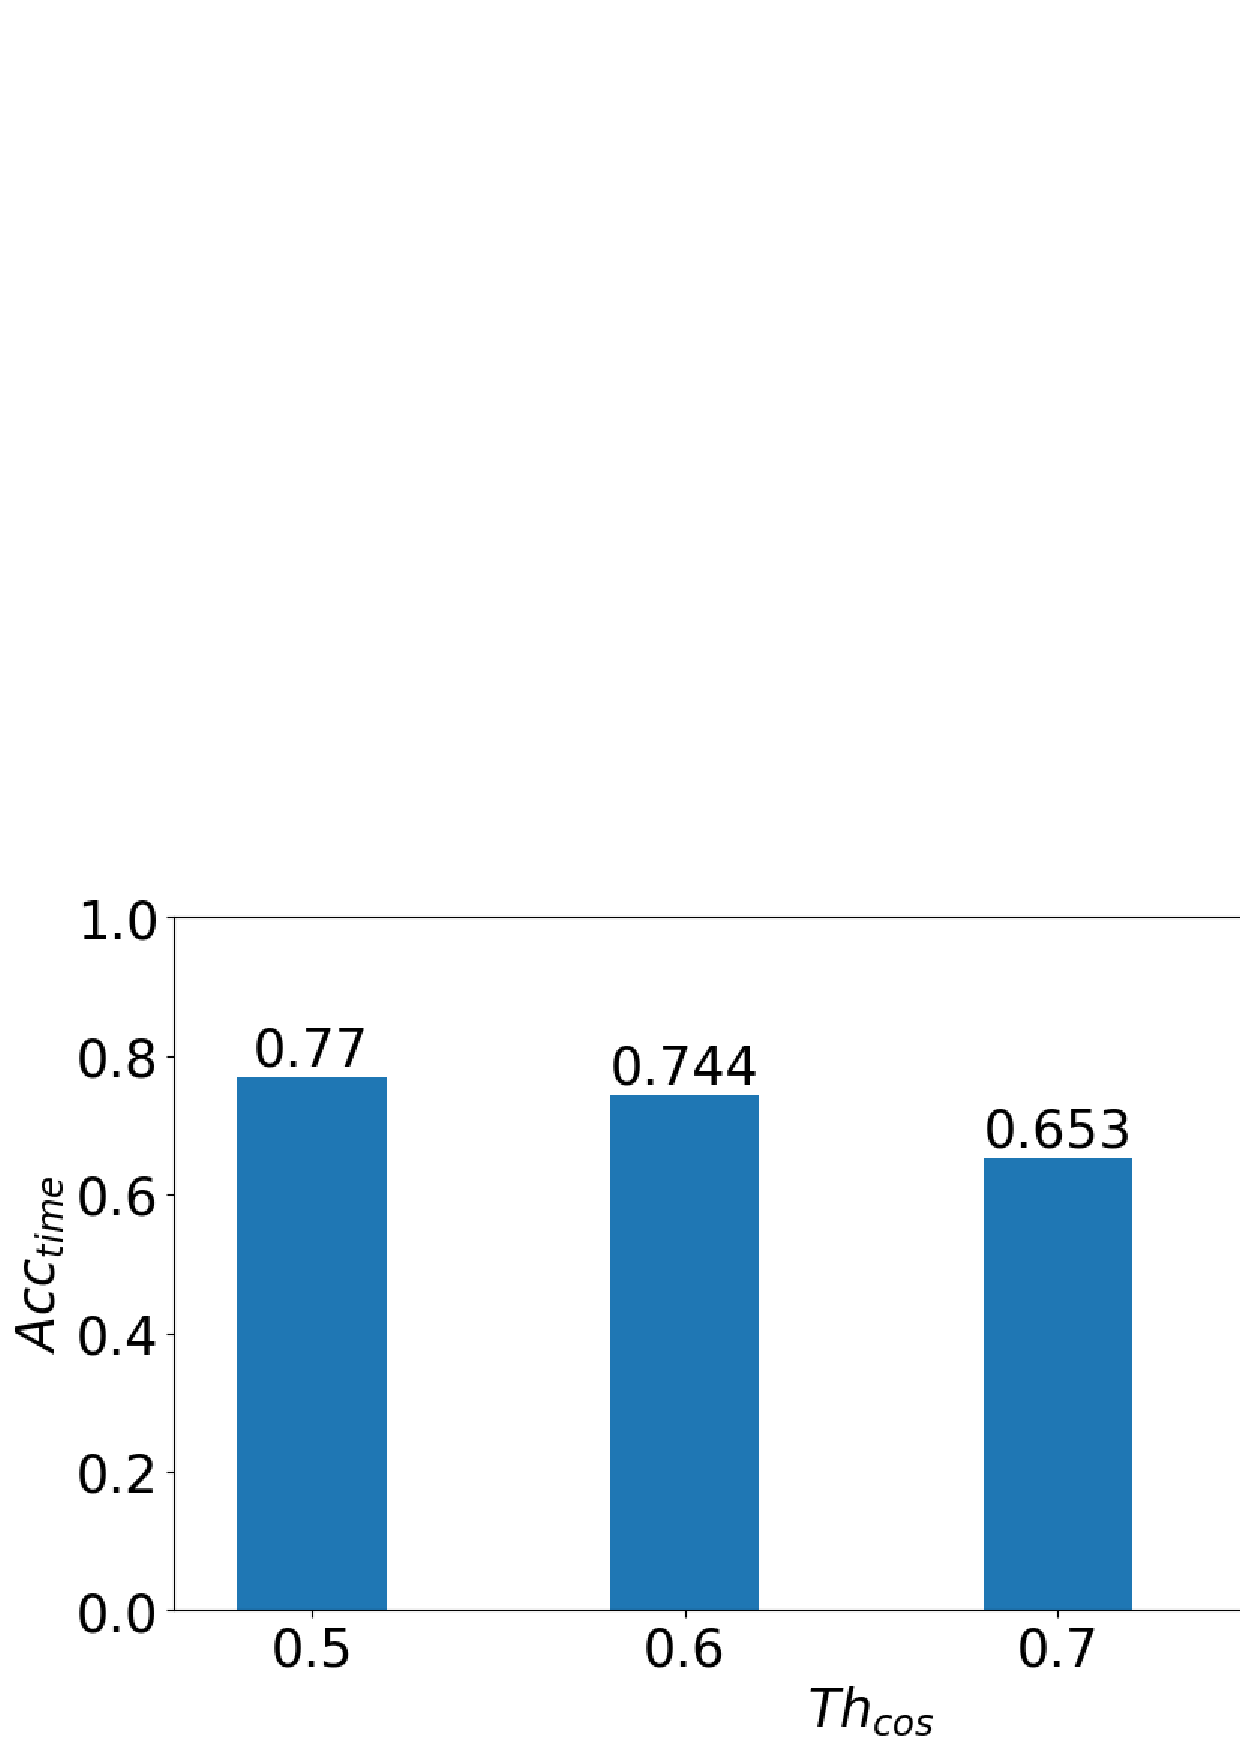
\includegraphics[keepaspectratio, scale=0.27]
                          {./figure/prob3_13_acc.eps}}
      \end{minipage}
    
    \end{tabular}
\caption{手法3によるアンカーの発話区間検出精度 ($Th_{time}=1.3$) \label{fig:result_anchor_prob3}}
\end{figure} 


\begin{table}[H]
  \begin{center}
    \caption{手法3による各ニュース番組音声のニュースアンカーの発話検出精度($Th_{cos}=0.6,Th_{time}=1.3$) \label{table:prob3_eachnews}}
    \begin{tabular}{|c||c|c|c|c|} \hline
データID & Recall & Precision & F-meature & 作成したクラスタ数\\ \hline
ニュース1 & 0.958 & 0.702 & 0.810 & 1 \\ \hline
ニュース2 & 0.758 & 0.590 & 0.663 & 2 \\ \hline
ニュース3 & 0.725 & 0.846 & 0.781 & 2 \\ \hline
ニュース4 & 0.646 & 0.755 & 0.696 & 2 \\ \hline
ニュース5 & 0.683 & 0.973 & 0.802 & 2 \\ \hline
    \end{tabular}
  \end{center}
\end{table}

実験の結果、Baselineを各手法を比較したとき、ニュースアンカーの検出精度の指標であるF-measureが手法1では6.5\%(図\ref{prob1_fmeasure})、手法2では2.3\%(図\ref{prob2_fmeasure})、手法3では4.7\%(図\ref{prob3_fmeasure})の向上が確認された。また、Baselineと提案手法の全てにおいてニュース2の検出精度であるPrecisionが最も低い。\par
いずれの手法においても$Th_{cos}$が小さい時にはRecallが高く、大きい時にはPrecisionが高くなる傾向が確認された。\par

\section{考察}
Baselineと提案手法を比較したとき提案手法のニュースアンカーの発話検出精度が最大で6.5\%向上したことから、結合した発話区間から抽出したi-vectorをニュースアンカーの検出に用いることは有効であることを示した。また、Baselineにおいて、$Th_{cos}$が0.8のとき、提案手法のみニュースアンカーの発話検出を行うことが出来たことから、i-vectorの抽出精度が向上したと考えることができる。\par
手法2と手法3の検出精度のF-measureが手法1と比較して低下した理由として、ニュースアンカーの発話中に流れるVTRの存在が挙げられる。話者が切り替わっていない場合であってもVTRに含まれる雑音や音楽が同時に流れることによって発話環境の変化と誤識別したため、発話区間の結合ができなかったためであると考えられる。\par
いずれの手法でもニュース2のニュースアンカーの発話検出精度であるP値が他のニュースと比較して低い理由として、表\ref{table:test_detail}や表\ref{table:num_of_anchor}で示されているように、アンカーの発話の割合が少ないことが挙げられる。本研究で用いたニュースアンカーの発話検出手法\cite{nozaki_gakuseikai}は、ニュースアンカーの発話の割合が多いことに着目して検出を行っている。そのため、ニュースアンカー以外の発話が多い話者の発話をニュースアンカーとして誤識別したためPrecisionが低下したと考えられる。\par
今後、発話数が少ないニュースアンカーの発話検出手法を検討することで、さらなるニュースアンカーの発話検出精度の向上が期待できると考えられる。\par
また、ニュースアンカーの発話検出精度の向上における音声認識への効果を検証するために、検出されたニュースアンカーの発話の音声認識実験を行った。音声認識システムの概要、実験の詳細を付録\ref{chapter:speech_recog}に記載する。音声認識実験の結果、インデクシングに十分な精度で音声認識が行われたとは言えないため、音声認識精度向上のために雑音除去や雑音に頑健な音声認識システムを構築する必要があると考えられる。
  % アンカーの発話群検出実験
%\section{アンカーの発話区間の音声認識実験}

\subsection{実験方法}
本実験では、\ref{section:yoshimura_pre_clustering}節で述べた話者クラスタを作成、音響モデルを作成して音声認識実験を行う。各話者クラスタに含まれる男女の発話データ数を図\ref{fig:yoshimura_kikouzou}に示す。

\begin{figure}[H]
  \begin{center}
    \includegraphics{./figure/kakiokosi.eps}
  \end{center}
  \caption{各話者クラスタに含まれる発話データ数 \label{fig:yoshimura_kikouzou}}
\end{figure}

本実験で使用した音響モデル、言語モデル、単語辞書の仕様は\ref{section:experiment_acoustic_model}節、\ref{section:experiment_language_model}節で述べる。

\subsection{音響モデルの仕様}
\label{section:experiment_acoustic_model}
本実験で用いたDNN-HMM音響モデルの仕様を表\ref{table:acoustic_model_detail}に示す。この仕様に関しては小島らの研究\cite{kojima}で使用されたもので、状態数は3000、音響特徴の次元数は39次元(表\ref{acoustic_model_feature})、隠れ層の数は6層、各層における繰り返し学習数は5回、隠れ層のノード数は1024とした。以下に、DNNを用いた際の学習の手順を示す。

\begin{table}[H]
  \begin{center}
    \caption{音響モデルの仕様 \label{table:acoustic_model_detail}}
    \begin{tabular}{|c|c|c|} \hline
     状態数  & 使用した音素 & 混合数 \\ \hline
     3,000  & 27 & 16 \\ \hline
    \end{tabular}
  \end{center}
\end{table}

\begin{table}[H]
  \begin{center}
    \caption{使用する音響特徴パラメータ \label{acoustic_model_feature}}
    \begin{tabular}{|c||c|} \hline
      特徴量 & 次元数\\ \hline
      MFCC & 12  \\ \hline
      POW & 1  \\ \hline
      $\Delta$MFCC & 12 \\ \hline
      $\Delta$POW & 1 \\ \hline
      $\Delta\Delta$MFCC & 12 \\ \hline
      $\Delta\Delta$POW & 1 \\ \hline
      計 & 39 \\ \hline
    \end{tabular}
  \end{center}
\end{table}

\vspace{0.2in}\noindent{\textbf{\underline{構築手順}}}\par
DNNを用いた音響モデルの構築や、この音響モデルを用いた音声認識に必要な学習テキストや言語モデルを作成する為にKaldiツールキットを用いた\cite{kaldi}。このツールキットの大きな流れを図\ref{fig:flow_train_dnn}に示す。まず学習や評価に必要なデータを用意し、言語モデルと単語辞書のWeighted Finite State Transducer (WFST)を作成する。WFSTとは重み付き有限トランスデューサといい、状態遷移機械モデル有限オートマトンの一種である。次に音声データから特徴量を抽出したデータを準備し、このデータと書き起こしを用いてGMM-HMMによる音響モデルのWFSTを作成する。これらのWFSTを、合成等を行ない1つのWFSTとする。このWFSTを用いて音声認識を行ない、学習データのアライメント(フレームごとの音素情報)をとる。このアライメントを用いてDNNを用いた音響モデルの学習(プレトレーニングと微調整)を行ない、最終的な音声認識を行なう。

\begin{figure}[H]
  \begin{center}
    \includegraphics{./figure/flow_train_dnn.eps}
  \end{center}
  \caption{DNNを用いる際の学習の流れ \label{fig:flow_train_dnn}}
\end{figure}

\vspace{0.2in}\noindent{\textbf{\underline{使用した音素}}}\par
本研究で使用した音素27個を表\ref{fig:used_onso}に示す。また、その音素をもとに記したカナ音素対応表を表\ref{fig:kana_onso}に示す


\begin{table}[H]
\begin{center}
\caption{使用した音素 \label{fig:used_onso}}
\begin{tabular}{|c|c|c|c|c|c|c|}
\hline
母音  & 子音         & 濁音  & 半濁音 & 撥音 & 促音 & 無音 \\ \hline
a i & ch f h j k & b d &     &    &    &    \\ 
u e & m n r s sh & g z & p   & ng & q  & \# \\ 
o   & t ts w     & zh  &     &    &    &    \\ \hline
\end{tabular}
\end{center}
\end{table}


\begin{table}[H]
  \begin{center}
    \caption{カナ音素対応表 \label{fig:kana_onso}}
    \includegraphics[scale=0.7]{./figure/kana_onso.eps}
  \end{center}
  
\end{table}

\subsection{言語モデル・単語辞書の仕様}
\label{section:experiment_language_model}
言語モデルはトライグラムモデルを構築した。以下、使用した学習テキストを説明する。

\vspace{0.2in}\noindent{\textbf{\underline{CSJ}}}\par
CSJには書き起こしテキストも提供されており、その一部の例を図\ref{fig:kakiokosi}に示す。書き起こしテキストは主に情報部と発話部に区別される。情報部では発話IDや時間情報等を、発話部では発話内容を「&」の左側に基本形、右側に発音形という形式で記している。発話形はカタカナを用いて実際に発音された音声を忠実に表記したものである。発音の怠けや言い間違い等を書き取れる範囲で忠実に記録している。本研究では、音響モデル構築の際には主に発話部の発音形を用い、このカタカナ表記を音素列に変換し、ラベルファイルとして定義する。
\begin{figure}[H]
  \begin{center}
    \includegraphics{./figure/kakiokosi.eps}
  \end{center}
  \caption{書き起こしテキストの例 \label{fig:kakiokosi}}
\end{figure}

本研究ではこのCSJをベースに学習テキストを構成する。使用するデータは977講演分のテキストで、約14MBである。

\vspace{0.2in}\noindent{\textbf{\underline{拡張したコーパスによる学習テキスト}}}\par
この学習テキストは江頭らによる、学術講演の書き起こしと新聞記事に拡張されるテキストとして参加者名の入ったテキスト、Webから収集してきたテキスト、そして対話コーパスから作成される対話テキストを追加した未知語の減少に着目した学習テキストである。この学習テキストは会議中に参加者の名前を呼ぶことが多い、会議は対話形式であるなどの会議の特徴を考慮した学習テキストである。テキストサイズは約100MBである。以降本論文では、このテキストを拡張したコーパスによる学習テキストと呼ぶ。

\vspace{0.2in}\noindent{\textbf{\underline{拡張したコーパスによる学習テキスト}}}\par
この学習テキストは荒井らによる、会議における発話行為に着目して作成された学習テキストである。学術講演の書き起こしと新聞記事に対話表現に近い特徴を持っていると考えられるQ&Aサイトから収集したテキストと対話コーパスを追加した学習テキストである。テキストサイズは約44MBである。以降本論文ではこのテキストを対話特化テキストと呼ぶ。


\subsection{評価方法}
本研究では評価尺度としては式\ref{calc:word_acc}で与えられる単語正解精度$Acc$(Word Accuracy)を用いる。ここで$W$は単語数、$S$(Substitution)は置換誤り、$D$(Deletion)は脱落誤り、$I$(Insertions)は挿入誤りの単語数を表わす。置換誤りとは、正解の単語が別の単語に誤認識された場合の誤りである。脱落誤りとは、単語があるべき部分に認識結果が何も出力されなかった場合の誤りである。挿入誤りは、本来単語がない部分に誤認識結果として単語が出力された場合の誤りである。

\begin{equation}
\label{calc:word_acc}
Acc=\frac{(W-S-D-I)}{W}
\end{equation}

          
評価は、正解ファイルと認識結果のファイルをDPマッチングを行なうことにより算出する。この正解ファイルは形態素解析した結果の形態素列によって作成したものである。


また、本研究ではアンカーの発話区間が既知の場合と未知の場合で音声認識精度の評価を行う。ここで、アンカーの発話区間が未知の時、\ref{chapter:get_anchor}節で検出したアンカーの発話区間のうち、各手法でもっともF値の高かった結果を対象とした音声認識を行うため、アンカー以外の発話区間で認識された単語は全て挿入誤り、アンカーの発話として検出出来なかった発話区間の単語は全て削除誤りとして計算する。
\subsection{実験結果}
\noindent{\textbf{\underline{アンカーの発話区間が既知の場合}}}\par
アンカーの発話区間が既知の場合の音声認識結果を表\ref{table:result_sprecog1}に示す。

\begin{table}[H]
  \begin{center}
    \caption{アンカーの発話区間が既知の場合の音声認識結果 \label{table:result_sprecog1}}
    \begin{tabular}{|c||c|c|c|c|c|} \hline
     手法  & $Acc$  & Substitution & Deletion & Insertions \\ \hline
     Baseline  & 61.6 & 463 & 307 & 1834 \\ \hline
     手法1  & 61.6  & 477 & 318 & 1813 \\ \hline
     手法2  & 61.7  & 460 & 305 & 1836\\ \hline
     手法3  & 61.6  & 460 & 304 & 1827 \\ \hline
    \end{tabular}
  \end{center}
\end{table}

Baselineと比較して、いずれの手法も認識精度の向上は確認できなかった。

\vspace{0.2in}\noindent{\textbf{\underline{アンカーの発話区間が未知の場合}}}\par
アンカーの発話区間が未知の場合の音声認識結果を表\ref{table:result_sprecog2}に示す。

\begin{table}[H]
  \begin{center}
    \caption{アンカーの発話区間が未知の場合の音声認識結果 \label{table:result_sprecog2}}
    \begin{tabular}{|c||c|c|c|c|c|} \hline
     手法  & $Acc$ & Word & Substitution & Deletion & Insertions \\ \hline
     Baseline  & 26.7  & 957 & 2334 & 1684 \\ \hline
     手法1  & 29.9  & 994 & 2080 & 1681 \\ \hline
     手法2  & 35.4  & 998 & 1713 & 1670\\ \hline
     手法3  & 35.4 & 998 & 1713 & 1670 & \\ \hline
    \end{tabular}
  \end{center}
\end{table}

アンカーの発話区間が未知の場合はいずれも発話区間が既知の場合と比較して大きく音声認識精度が低下した。また、いずれの手法もBaselineと比較して音声認識精度は向上している。
\subsection{考察}
アンカーの発話区間が既知の場合に音声認識精度がいずれも変化がなかった理由として、背景雑音、音楽の存在が考えられる。これは、音響モデルの学習に用いたCSJが声の入らない環境で収録を行っているため、雑音、音楽が同時になった状態の音声は収録されていない。このため、本実験で作成した木構造話者クラスの音響モデルのいずれも認識できない発話が多く存在してしまい、認識精度の違いがなかったと考えられる。そのため、音声認識精度の向上のために、雑音除去、もしくは雑音、音楽に頑健な音響モデルの作成が必要であると考えらえる。\par
アンカーの発話区間が未知の場合はいずれも発話区間が既知の場合と比較して大きく音声認識精度が低下した理由として、アンカー以外の発話区間で認識された単語は全て挿入誤り、アンカーの発話として検出出来なかった発話区間の単語は全て削除誤りとして計算したためである。また、いずれの手法もBaselineと比較してアンカーの発話区間検出精度が向上していたため、音声認識精度はいずれの手法もBaselineと比較して音声認識精度は向上している。
  % 音声認識実験
\chapter{結論}
本研究では、ニュース番組音声のインデクス自動付与に向けたダイアライゼーション実現のために、i-vectorを用いたニュースアンカーの発話検出精度向上を目指した。\par

i-vectorは短い発話データから話者の識別に必要な話者の特徴を表現することが難しく、ニュースアンカーの発話検出精度の低下の原因となっているため、本研究では短い発話に着目してニュースアンカーの発話検出を高精度に行うことを目的とした。\par

本研究ではニュース番組における「発話の時間間隔」と「発話環境」の二点を考慮した手法を提案し、ニュースアンカーの発話検出精度への有効性を検証した。一つ目に、同一話者が連続で発話する場合、発話と発話の間の時間間隔が非常に短くなることに着目した。つまり、発話間の時間が非常に短いとき前後の発話が同一話者の可能性が高いと考え、発話区間の結合を行うことで擬似的に長い発話を作成した。二つ目に、スタジオにいるニュースアンカーや、屋外でインタビューを受けるインタビューイなど、様々な環境で話者が発話していることに着目した。発話者の発話環境を検出するために音源識別を行い、前後の発話の発話者の発話環境が同じである可能性が高いとき同一話者であると考え、発話区間の結合を行った。以上の2通りの手法で結合した発話区間から抽出したi-vectorを用いて、ニュースアンカーの発話検出を行った。\par

ニュースアンカーの検出精度の評価指標であるF値を従来手法と比較したところ、発話の時間間隔を考慮した手法が6.5\%、発話環境を考慮した手法が2.3\%の検出精度向上が確認された。また、両方の手法を組み合わせて実験を行ったところ、従来手法と比較して4.7\%の検出精度の向上が確認されたが、発話の時間間隔のみを考慮した場合と比較すると精度が1.8\%低下した。またいずれの手法も、ニュースアンカーの発話数が少ないニュース番組の発話検出精度のP値がニュースアンカーの発話数が多いニュース番組と比較して、10\%程度低下した。\par

いずれの提案手法を用いた場合でも、従来手法と比較してニュースアンカーの発話検出精度が向上したことから、発話区間の結合は話者の特徴抽出とニュースアンカーの発話検出に有効であると考えられる。また、発話間隔を考慮した手法と発話環境を考慮した手法で発話検出精度に差が生じた理由として、ニュースアンカーの発話中に流れるVTRや中継映像の存在が考えられる。VTRや中継映像には音楽や雑音が含まれていることから、ニュースアンカーがスタジオで発話していた場合であっても、音源識別結果を用いた場合発話環境が変化したと誤認識する。以上の理由により、同一話者間の発話であっても発話の結合が出来なかった箇所が存在するため、i-vectorがニュースアンカーの検出に必要な話者の特徴を抽出できなかったと考えられる。また、ニュースアンカーの発話数によって発話の検出精度が低下した理由として、本研究で用いたニュースアンカーの発話検出手法がニュース番組内において、ニュースアンカーの発話が非常に多いことに着目した手法であるためである。このため、発話の少ないニュースアンカーの発話を十分に検出できず、検出精度が低下したと考えられる。\par
今後、ニュースアンカーの発話数に依らないニュースアンカーの発話検出手法を提案することで、発話検出精度の改善が期待できる。

\begin{comment}
本稿では、ニュース番組音声のインデクス自動付与に向けたダイアライゼーション実現のために、発話間隔と発話環境を考慮したi-vectorを用いたニュースアンカーの発話検出精度向上を目指した。\par
特定話者の識別にはi-vectorが一般的に用いられるが、短い発話からは話者の識別に必要な十分な話者の特徴を抽出できない。そのため、本稿では前後の発話区間が同一話者の発話である可能性が高いとき発話区間を結合し、長い発話を擬似的に作成した。次に、結合した発話区間からi-vectorを抽出することで短い発話から得られるi-vectorの抽出精度向上を目指した。発話区間の結合には、同一話者が連続で発話する場合間をおかずに発話すること、話者が切り替わった時に発話環境が変化することに着目し、発話と発話の時間間隔を考慮する手法と、発話者の発話環境を考慮する手法を用いた。以上の手法を用いて結合した発話区間から抽出したi-vectorを用いてニュースアンカーの発話検出を行った結果、発話検出精度が約6\%向上し、ニュースアンカーの発話検出への有意性を示した。しかし、ニュースアンカーの発話数が少ないニュース番組においてはアンカーの検出精度が著しく低下した。このため、ニュースアンカーの発話が少ない場合においても発話を検出する手法を提案する必要がある。\par
また、本研究で抽出したi-vectorを用いてニュースアンカーの音声認識を行なった。音声認識はニュースアンカーの発話区間が既知の場合と未知の場合で行い、発話区間が既知のときは音声認識精度の向上が確認できなかった。ニュースアンカーの発話区間が未知の場合、従来と比較してニュースアンカーの発話区間検出精度が向上したことが音声認識精度の向上に繋がった。\par
今後の課題として、ニュースアンカーの発話が少ない番組におけるニュースアンカーの発話検出精度の向上が必要である。これは、発話内容などi-vector以外のニュースアンカーの特徴を考慮する必要があると考えられる。また、音声認識においては、ニュース音声の背景雑音の除去、雑音に頑健な音響モデルの作成が挙げられる。ニュースアンカーはスタジオで発話しているため基本的には音声以外は入らないが、参考映像などの音が発話中に流れることがある。そのため、雑音、音楽に対して音源分離による雑音除去や、雑音や音楽が含まれた学習データを用いて音響モデルを学習することで、音声認識精度が向上すると考えられる。
\end{comment}  % まとめ
\chapter*{謝辞}

最後に,本研究および本修士論文作成にあたり暖かい御指導および適切な御助言をして頂いた松永 昭一教授,高田 寛之助教,山下 優博士に心より感謝いたします.

また,同研究室
博士前期(修士)課程2年の三浦 亮氏,
博士前期(修士)課程1年の入口 佳佑氏,堤 彬人氏,福永 慶士氏,
学士課程4年の平野 吉則氏,Zhang Tianzhi氏,
阿利 迪洋氏,梅野 直幹氏,古賀 光氏,増田 紗依氏,松本 優里奈氏,その他関係各位に心から感謝いたします.
    % 謝辞
\addcontentsline{toc}{chapter}{謝辞}
\begin{thebibliography}{99}     %文献数が10未満の時 {9}
\bibitem{yamaguchi_indexing}山口 正秀,松永昭一,山下優,"Spectral Cross-Correlation Features for Audio Indexing of Broadcast News and Meetings",Eurospeech,pp613-615(2005)
\bibitem{yoshimura_clustering}吉村竜哉,"話者クラスタ音響モデルを用いた会議音声認識のための話者適応",電気情報通信学会九州支部学生会講演会(2014)
\bibitem{iv}N.Dehak, P.Kenny, R.Dehak, P.Dumouchel and P.Ouellet,"Front-end factoranalysis forspeaker verifiCatiOn" IEEE Trans. Audio Speech Lang. Process, 19, 788-798(2011)
\bibitem{nozaki_gakuseikai}野崎大智,"ニュース音声におけるi-vectorを用いた同一アンカーの発話群の検出",電気情報通信学会九州支部学生会講演会(2018)
\bibitem{adachi_gakuseikai}安達大輔,"ニュース番組における発話者群の段階的分類の検討",電気情報通信学会九州支部学生会講演会(2012)
\bibitem{panaiv}辻川美沙貴,西川剛樹,松井知子,"i-vectorによる短い発話の話者識別の検討",電子情報通信学会(2015)
\bibitem{ATR}国立情報学研究所データセット集合利用研究開発センター"ATRバランス文"
\bibitem{alize}"ALIZE",http:/alize.univ-avignon.fr
\bibitem{shimae_9}冨久祐介,“音源識別のための音クラスタリングとガウス分布混合数の有効性の検討”,
長崎大学工学部情報システム工学科平成,19年度卒業論文(2008)
\bibitem{shimae_10}水野理, 大附克年, 松永昭一, 林良彦: “ニュースコンテンツにおける音響信号自動判
別の検討”, 電気情報通信学会総合大会(2003)
\bibitem{sp_recognition_shikano}:鹿野清宏,伊藤克亘,河原達也,武田一哉,山本幹雄,"音声認識システム",情報処理学会,オーム社(2003)
\bibitem{audio_textbook}河原達也,"音声認識システム",情報処理学会(2016)
\bibitem{kaldi}"KALDI",http://kaldi.sourceforge.net/
\bibitem{kojima}小島和也,"会議音声認識のためのDNNを用いた高精度な音響モデルの構築法の検討",長崎大学工学部情報システム工学科 平成25年度修士論文(2013)
\bibitem{egashira_text}江頭一茂,"会議の発話分の特徴に合わせた会議音声認識用言語モデルの構築法の検討",長崎大学工学部情報システム工学科,平成25年修士論文(2013)
\bibitem{arai_text}荒井勇吏,"会議音声認識のための発話行為依存言語モデルの構築",長崎大学工学部情報システム工学科,平成26年修士論文(2014)
\bibitem{shimae_11}新美康永,“音声認識”,共立出版株式会社(1979)
\end{thebibliography}
    % 参考文献
\addcontentsline{toc}{chapter}{参考文献} 

% 付録がある場合
%\appendix
%\input{app}    % 付録

\end{document}
